% arara: pdflatex: { synctex: true, shell: true}   
% arara: bibtex
% arara: pdflatex: { synctex: true, shell: true}

%
% uaThesis example (for a thesis written in Portuguese)
%
% the complete list of options and commands can be found in uaThesis.sty
%
%

\documentclass[11pt,twoside,a4paper]{report}
\usepackage[DETI,newLogo]{uaThesis}

\def\ThesisYear{2018}

% optional packages
\usepackage[UKenglish]{babel}
\usepackage{multicol}
\usepackage{acronym}
\usepackage[acronym, toc, automake]{glossaries}
\usepackage{hyperref}
\usepackage{epsfig}     
\usepackage{subfig} 
\usepackage{amsmath}
\usepackage{amssymb}
\usepackage{listings}
\usepackage{color}
\usepackage{fancyvrb}
\usepackage{ifthen}
\usepackage{texments}
\usepackage{fancyhdr}
\usepackage{xspace}% used by \sigla

\usepackage[
backend=biber,
style=alphabetic,
citestyle=authoryear
]{biblatex}

\addbibresource{library.bib} %Imports bibliography file


\definecolor{mygreen}{rgb}{0,0.6,0}
\definecolor{mygray}{rgb}{0.5,0.5,0.5}
\definecolor{mymauve}{rgb}{0.58,0,0.82}


\lstset{ %
	backgroundcolor=\color{white},   % choose the background color; you must add \usepackage{color} or \usepackage{xcolor}; should come as last argument
	basicstyle=\fontfamily{sbc}\selectfont,        % the size of the fonts that are used for the code
	breakatwhitespace=false,         % sets if automatic breaks should only happen at whitespace
	breaklines=true,                 % sets automatic line breaking
	captionpos=b,                    % sets the caption-position to bottom
	commentstyle=\color{mygreen},    % comment style
	deletekeywords={...},            % if you want to delete keywords from the given language
	escapeinside={\%*}{*)},          % if you want to add LaTeX within your code
	extendedchars=true,              % lets you use non-ASCII characters; for 8-bits encodings only, does not work with UTF-8
	%frame=single,	                   % adds a frame around the code
	keepspaces=true,                 % keeps spaces in text, useful for keeping indentation of code (possibly needs columns=flexible)
	keywordstyle=\color{blue},       % keyword style
	%  language=XML,                 % the language of the code
	morekeywords={*,...},            % if you want to add more keywords to the set
	numbers=left,                    % where to put the line-numbers; possible values are (none, left, right)
	numbersep=5pt,                   % how far the line-numbers are from the code
	numberstyle=\tiny\color{mygray}, % the style that is used for the line-numbers
	rulecolor=\color{black},         % if not set, the frame-color may be changed on line-breaks within not-black text (e.g. comments (green here))
	showspaces=false,                % show spaces everywhere adding particular underscores; it overrides 'showstringspaces'
	showstringspaces=false,          % underline spaces within strings only
	showtabs=false,                  % show tabs within strings adding particular underscores
	stepnumber=1,                    % the step between two line-numbers. If it's 1, each line will be numbered
	stringstyle=\color{mymauve},     % string literal style
	tabsize=2,	                   % sets default tabsize to 2 spaces
}

\lstdefinestyle{xml}{
	belowcaptionskip=1\baselineskip,
	breaklines=true,
	%  frame=L,
	%  xleftmargin=\parindent,
	language=XML,
	showstringspaces=false,
	basicstyle=\footnotesize\ttfamily,
	keywordstyle=\bfseries\color{green!40!black},
	commentstyle=\itshape\color{purple!40!black},
	identifierstyle=\color{blue},
	stringstyle=\color{orange},
}

\definecolor{maroon}{rgb}{0.5,0,0}
\definecolor{darkgreen}{rgb}{0,0.5,0}
\lstdefinelanguage{XML}
{
	basicstyle=\ttfamily,
	morestring=[s]{"}{"},
	morecomment=[s]{?}{?},
	morecomment=[s]{!--}{--},
	commentstyle=\color{darkgreen},
	moredelim=[s][\color{black}]{>}{<},
	moredelim=[s][\color{red}]{\ }{=},
	stringstyle=\color{blue},
	identifierstyle=\color{maroon}
}

\makeglossaries
\glstoctrue

\newacronym{ad}{AD}{Autonomous Driving}
\newacronym{adas}{ADAS}{Advanced Driver Assistance Systems}
\newacronym{ros}{ROS}{Robot Operating System}
\newacronym{gui}{GUI}{Graphical User Interface}
\newacronym{pcl}{PCL}{Point Cloud Library}
\newacronym{opencv}{OpenCV}{Open Source Computer Vision Library}
\newacronym{lidar}{LIDAR}{Light Detection And Ranging}
\newacronym{lar}{LAR}{Laboratory of Automation and Robotics}
\newacronym{mtt}{MTT}{Multi Target Tracking}
\newacronym{hsv}{HSV}{Hue, Saturation and Value}
\newacronym{rca}{RCA}{Radio Corporation of America}
\newacronym{atc}{ATC}{Advanced Technologies Center}
\newacronym{darpa}{DARPA}{Defense Advanced Research Projects Agency}
\newacronym{scot}{SCOT}{Shared Computer-Operated Transit}
\newacronym{smart}{SMART}{Singapore-MIT Alliance for Research and Technology}
\newacronym{kitti}{KITTI}{Karlsruhe Institute of Technology
	and Toyota Technological Institute}
\newacronym{mpii}{MPII}{Max Planck Institut Informatik}
\newacronym{ethz}{ETHZ}{Eidgenössische Technische Hochschule Zürich}
\newacronym{epfl}{EPFL}{\'Ecole polytechnique f\'ed\'erale de Lausanne}
\newacronym{roi}{ROI}{Region of Interest}
\newacronym{lartk}{LARTk}{\gls{lar} Toolkit}

% optional (comment to use default)s
%   depth of the table of contents
%     1 ... chapther and sections
%     2 ... chapters, sections, and subsections
%     3 ... chapters, sections, subsections, and subsubsections
\setcounter{tocdepth}{3}

% optional (comment to used default)
%   horizontal line to separate floats (figures and tables) from text
\def\topfigrule{\kern 7.8pt \hrule width\textwidth\kern -8.2pt\relax}
\def\dblfigrule{\kern 7.8pt \hrule width\textwidth\kern -8.2pt\relax}
\def\botfigrule{\kern -7.8pt \hrule width\textwidth\kern 8.2pt\relax}

% custom macros (could also be defined using \newcommand)
\def\I{\mathtt{i}}         % one possible way to represent $\sqrt{-1}$
\def\Exp#1{e^{2\pi\I #1}}  % argument inside braces, i.e., "{}"
\def\EXP#1.{e^{2\pi\I #1}} % argument finishes when a full stop is encountered, i.e., "."
\def\sigla{\LaTeX\xspace}  % use as "blabla \sigla blabla (no need to do "blabla \sigla\ blabla"

\def\AddVMargin#1{\setbox0=\hbox{#1}%
                  \dimen0=\ht0\advance\dimen0 by 2pt\ht0=\dimen0%
                  \dimen0=\dp0\advance\dimen0 by 2pt\dp0=\dimen0%
                  \box0}   % add extra vertical space above and below the argument (#1)
\def\Header#1#2{\setbox1=\hbox{#1}\setbox2=\hbox{#2}%
           \ifdim\wd1>\wd2\dimen0=\wd1\else\dimen0=\wd2\fi%
           \AddVMargin{\parbox{\dimen0}{\centering #1\\#2}}} % put #1 on top #2



\begin{document}

%
% Cover page (use only one of the first two \TitlePage)
%

% First alternative, with a figure
\TitlePage
  %\GRID  % for debugging ONLY
  \HEADER{\BAR\FIG{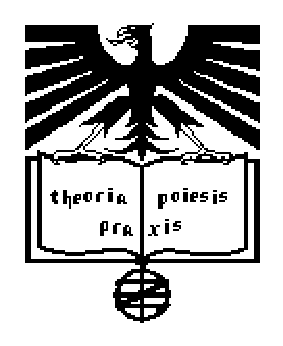
\includegraphics[height=60mm]{uaLogoOld}}} % the \FIG{} is optional
         {\ThesisYear}
  \TITLE{Nuno Miguel \newline Soares Silva}
        {Perce\c c\~ao Aumentada para o AtlasCar \newline Augmented Perception for AtlasCar}
\EndTitlePage
\titlepage\ \endtitlepage % empty page

%
% Initial thesis pages
%

\TitlePage
  \HEADER{}{\ThesisYear}
  \TITLE{Nuno Miguel \newline Soares Silva}
        {Perce\c c\~ao Aumentada para o AtlasCar \newline Augmented Perception for AtlasCar}
  \vspace*{15mm}
  \TEXT{}
       {Disserta\c c\~ao apresentada \`a Universidade de Aveiro para cumprimento dos requesitos
        necess\'arios \`a obten\c c\~ao do grau de Mestre em Engenharia de Computadores e Telem\'atica , realizada sob a orienta\c c\~ao
        cient\'\i fica de Paulo Miguel de Jesus Dias, Professor Auxiliar do Departamento de Electr\'onica, Telecomunica\c c\~oes e Inform\'atica da Universidade de Aveiro, de Vitor Manuel Ferreira dos Santos, Professor Associado do Departamento de Engenharia Mec\^ anica e de Miguel Armando Riem de Oliveira, Professor Auxiliar do Departamento de Engenharia Mec\^ anica.}
\EndTitlePage
\titlepage\ \endtitlepage % empty page

\TitlePage
  \vspace*{55mm}
  \TEXT{\textbf{o j\'uri~/~the jury\newline}}
       {}
  \TEXT{presidente~/~president}
       {\textbf{Prof. Doutor A}\newline {\small
        Professor Catedr\'atico da Universidade de Aveiro (por delega\c c\~ao da Reitora da
        Universidade de Aveiro)}}
  \vspace*{5mm}
  \TEXT{vogais~/~examiners committee}
       {\textbf{Prof. Doutor B}\newline {\small
        Professor Catedr\'atico da Universidade de Aveiro (orientador)}}
  \vspace*{5mm}
  \TEXT{}
       {\textbf{Prof. Doutor C}\newline {\small
        Professor associado da Universidade J (co-orientador)}}
\EndTitlePage
\titlepage\ \endtitlepage % empty page

\TitlePage
  \vspace*{55mm}
  \TEXT{\textbf{agradecimentos~/\newline acknowledgements}}
       {\'E com muito gosto que aproveito esta oportunidade para agradecer a todos os que me
        ajudaram durante este longos e penosos anos, cheios de altos e baixos (mais baixos que
        altos)\ldots}
  \TEXT{}
       {Desejo tamb\'em pedir desculpa a todos que tiveram de suportar o meu desinteresse pelas
        tarefas mundanas do dia-a-dia, \ldots}
\EndTitlePage
\titlepage\ \endtitlepage % empty page

\TitlePage
  \vspace*{55mm}
  \TEXT{\textbf{Palavras-chave}}
  {Navega{\c c}\~ao aut\'onoma; ATLASCAR; Agrupamento de dados; Calibra{\c c}\~ao; Etiqueta\c c\~ao de dados; Dete\c c\~ao de Objetos; ADAS.}
  \vspace*{5mm}
  \TEXT{\textbf{Resumo}}
       {Este trabalho baseia-se no desenvolvimento de um pacote ROS para o ATLASCAR 2. O ATLASCAR 2 consiste em um Mitsubishi i-MiEV usado exclusivamente para investiga\c c\~ao de sistemas avan\c cados de assist\^encia \`a condu\c c\~ao no Departamento de Engenharia Mec\^anica da Universidade de Aveiro. O ATLASCAR 2 est\'a equipado com uma c\^amera PointGrey que foi usada para aquisi\c c\~ao de imagens, dois scanners planares LIDAR e um laser de quatro feixes frontais. Este pacote ROS implementa n\'os para dete\c c\~ao semi-autom\'atica de objetos. Estes n\'os s\~ao ut\'eis para etiquetar os dados ligados aos objetos detetados. Estes objetos, na pr\'atica, ser\~ao por exemplo ve\'iculos e pe\~oes na estrada. A manipula\c c\~ao dos dados na imagem foi realizada atrav\'es das bibliotecas de OpenCV. Em paralelo, foi desenvolvido e melhorado a dete\c c\~ao da bola para o pacote de calibra\c c\~ao multi-sensorial.
       	}
\EndTitlePage
\titlepage\ \endtitlepage % empty page

\TitlePage
  \vspace*{55mm}
  \TEXT{\textbf{Keywords}}
  {Autonomous driving; ATLASCAR; Data Clustering; ; Calibration; Data Labelling; Object Detection; ADAS.}
  \vspace*{5mm}
  \TEXT{\textbf{Abstract}}
       {This thesis is based on the development of a ROS package for the ATLASCAR 2. The ATLASCAR 2 consists in a Mitsubishi i-MiEV used exclusively for research of Advanced driver assistance systems (or ADAS) in the Mechanical Engineering Department at University of Aveiro. The ALTASCAR 2 is equipped with a PointGrey camera used to acquire images, two planar LIDAR scanners and a four-beam frontal scanner. This ROS package implements nodes for semi-automatic object detection. This nodes are useful to label data to the detected objects. This objects, in practice, are for example vehicles or pedestrians on the street. The handling of the image data was done through OpenCV libraries. In parallel, it was developed and improved the ball detection for the multi-sensorial calibration package.
       	}
\EndTitlePage
\titlepage\ \endtitlepage % empty page


%
% Tables of contents, of figures, ...
%

\pagenumbering{roman}
\tableofcontents

\cleardoublepage
\listoffigures

\cleardoublepage
\listoftables

\clearpage
\chapter*{Acronyms}

\begin{multicols}{2}
	\begin{acronym}[AAAAAA]

		\acro{AD}{Autonomous Driving}
		\acro{ADAS}{Advanced Driver Assistance Systems}
		\acro{ROS}{Robot Operating System}
		\acro{GUI}{Graphical User Interface}
		\acro{PCL}{Point Cloud Library}
		\acro{OpenCV}{Open Source Computer Vision Library}
		\acro{LIDAR}{Light Detection And Ranging}
		\acro{LAR}{Laboratory of Automation and Robotics}		
		\acro{LARTk}{\gls{lar} Toolkit}
		\acro{MTT}{Multi Target Tracking}
		\acro{HSV}{Hue, Saturation and Value}
		\acro{RCA}{Radio Corporation of America}
		\acro{ATC}{Advanced Technologies Center}
		\acro{DARPA}{Defense Advanced Research Projects Agency}
		\acro{SCOT}{Shared Computer-Operated Transit}
		\acro{SMART}{Singapore-MIT Alliance for Research and Technology}
		\acro{KITTI}{Karlsruhe Institute of Technology
			and Toyota Technological Institute}
		\acro{MPII}{Max Planck Institut Informatik}
		\acro{ETHZ}{Eidgenössische Technische Hochschule Zürich}
		\acro{EPFL}{\'Ecole polytechnique f\'ed\'erale de Lausanne}
		\acro{ROI}{Region of Interest}
	\end{acronym}
\end{multicols}




% The chapters (usually written using the isolatin font encoding ...)

\titlepage\ \endtitlepage      % Página de verso em branco
\pagenumbering{arabic}


% ----------------------------------------------------------------
% Definicao de headers e footers
% ----------------------------------------------------------------
\pagestyle{fancy}
\renewcommand{\chaptermark}[1]{\markboth{\thechapter.#1}{}} % Capítulos em minúsculas
\fancyhf{}                                                  % Reset aos headers e footers
\fancyhead[LE,RO]{\thepage}                               % Header Left-Even (LE), Right-Odd (RO)
\fancyhead[LO]{\leftmark}                                 % Header Left-Odd (LO)
\fancyhead[RE]{\leftmark}                                 % Header Right-Even (RE)
\fancyfoot[LE]{Nuno Miguel Soares Silva}                               % Footer Left-Even (LE)
\fancyfoot[LO]{Nuno Miguel Soares Silva}                               % Footer Left-Odd (LO)
\fancyfoot[RE]{\textit{Master's thesis}}     % Footer Right-Even (RE)
\fancyfoot[RO]{\textit{Master's thesis}}     % Footer Right-Odd (RO)
\renewcommand{\headrulewidth}{0.25pt}                     % Espessura da linha de header
\renewcommand{\footrulewidth}{0.25pt}                     % Espessura da linha de footer
\addtolength{\headheight}{0.5pt}                          % Espaçamento para a linha

\chapter{Introduction}
Technological studies in the fields of \gls{adas} and \gls{ad} have been growing in the past decades in the auto-mobile industry and in the academic environment. 

It is important in \gls{ad} and \gls{adas} to implement machine learning methods so that the vehicles recognize what objects are in their surroundings. Therefore, a necessity to have data that instructs the vehicles appears. Data labelling is the solution to create datasets that will serve as input to learning algorithms.

This thesis is focused on the research of a method to label data into labels using a camera and \gls{lidar} sensors in ATLASCAR 2, so that the vehicle can later create a model of the objects it will detect, track and label.

The objects detected by ATLASCAR 2 are to be used in deep-learning algorithms. The acquired data must be large enough so that the models for each object can be well defined.

This dissertation will also improve some previous work, namely the calibration of the camera installed in ATLASCAR 2. In addition to the calibration, a tool for image labeling and tracking of objects will be developed. This tool will be used to gather image templates while tracking objects in the camera video. 

\section{ATLAS Project}

ATLAS is a project developed by the Group of Automation and Robotics at the Department of Mechanical Engineering of the University of Aveiro, Portugal. The mission of the ATLAS project is to develop and enable the proliferation of advanced sensing and active systems designed for implementation in automobiles and affine platforms. Advanced active systems being improved, or newly developed, use data from vision, laser and other sensors. The ATLAS project has vast experience with autonomous navigation in controlled environments and is now evolving to deal with real road scenarios. To ensure that the developments are meeting the ATLAS project mission statement, a full sized prototype, the ATLASCAR 1, has been equipped with several state of the art sensors. \cite{LARlabs} Currently, ATLASCAR 2 is the new full sized prototype being used for research. The ATLASCAR 2 is also equipped with \gls{lidar} sensors and a camera.

\subsection{History}

The ATLAS Project was created in 2003 and began with robots developed to participate at \gls{ad} competitions taking place at Portuguese National Robotics Festival. From this project, three small-sized platform robots were built (figure \ref{fig:atlasproto}). These robots were very successful having won prizes in some of the robotics competitions. 


\begin{figure}[htp]
	
	\centering
	\includegraphics[width=.3\textwidth]{capintro/imgs/atlas1}\hfill
	\includegraphics[width=.3\textwidth]{capintro/imgs/atlas2000}\hfill
	\includegraphics[width=.3\textwidth]{capintro/imgs/atlasmv}
	
	\caption{ATLAS project small-sized prototypes}
	\label{fig:atlasproto}
	
\end{figure}

As the project grew, it has evolved into full-sized prototypes: the ATLASCARs. ATLASCAR 1 (figure \ref{fig:atlascar1}) is the first full-sized platform and it is based on a Ford Escort Station Wagon. The ATLASCAR 1 is well equipped with several \gls{lidar} sensors and a camera. Data about its environment is gathered by the scanners which is then processed building perception into the car. With perception is possible for the vehicle to actuate allowing the car to move autonomously. 

\begin{figure}[htp]
	
	\centering
	\includegraphics[width=0.9\textwidth]{capintro/imgs/atlascar1}
	
	\caption{ATLASCAR 1 based on the Ford Escort platform}
	\label{fig:atlascar1}
	
\end{figure}

The ATLASCAR 1 brought successful results. In the end, the vehicle was able to move and execute maneuvers autonomously in small and controlled places. The ATLASCAR 1 was then replaced by a more recent vehicle. The ATLASCAR 2 (figure \ref{fig:atlascar1}) is the new full-sized platform of the ATLAS project and it is based on a Mitsubishi i-MiEV. This is the vehicle used for research in this dissertation. The ATLASCAR 2 is well equipped with various \gls{lidar} sensors and a camera. It is also a full electric vehicle which will be easier to modify, test and control. 

\begin{figure}[htp]
	
	\centering
	\includegraphics[width=0.9\textwidth]{capintro/imgs/imiev}
	
	\caption{Mitsubishi i-MiEV platform where ATLASCAR 2 is based}
	\label{fig:atlascar2}
	
\end{figure}


\section{Motivation}
The ATLASCAR 2 is the new platform of the ATLAS Project. The car has a mounted infrastructure for \gls{lidar} scanners and a vision-based sensors. With a fully equipped vehicle, the data from the surroundings is ready to be received and processed. 

To use multiple sensors at the same time in a system, it is fundamental that these devices are properly calibrated. The LIDAR sensors and the camera can be submitted into an extrinsic calibration in order to find their position relatively to a reference sensor. A fully calibrated system is important to deal with the data acquired from each sensor. Planar LIDAR sensors need to know their position between each other so that a full pointcloud of all sensors can be created for visualization purposes or for any end.

\gls{ad} and \gls{adas} often make use of machine learning. Deep learning algorithms utilize neural and convolutional networks for images and range-based sensor data. In the fields of machine learning, images are often used as input templates to create object models. In an image sequence it is possible to track an object and obtain samples of the \gls{roi} where the target is. This way it is possible for an algorithm to automatically recognize an object.

While registering the position of the objects in an image sequence, it is important to tell what those objects are. Labelling is the act to classify objects in a certain group. As the annotation is done, when selecting an object, the user should enter a label that identifies the target making it easy for the learning algorithm to recognize to object afterwards.

The objective and importance of tagging samples of images with a label is to assign metadata in the form of a keyword in order that later an application can retrieve this information and easily construct a database. However, most labelling for images is currently done with non optimized rudimentary procedures like capturing samples of the \gls{roi} manually and frame by frame, making this process slow and obsolete.

In the end of this dissertation, the ATLASCAR2 will have a labelling system that fuses images retrieved from the camera with the laser data, creating a semi automatic object tracking system that offers the possibility to retrieve various image template sequences and store metadata about them. This metadata contains, for instance, the label, object related identification markers and position of the object in the image and in the real world relatively to the ATLASCAR2.

\section{Objectives}
The objectives for this dissertation are, firstly, to improve the calibration of the camera, in particular regarding the detection of the ball by the camera in the existing multi-sensor calibration package developed using the \gls{ros}. Secondly, the development of other \gls{ros} package used for semi-automatic detection and labelling of objects in the field of view.

The calibration package was already developed by \cite{VieiradaSilva2016}. The methods used to detect the ball in the camera image were basically filtering values from the \gls{hsv} color space. There are methods that can make this detection more robust that will be explained in this thesis. 

To complete the goal of object tracking and image labelling there were a set of techniques and libraries used. In vision-based sensors, the object tracking algorithm is based on template matching methods and in range-based sensors the tracking is accomplished by the \gls{mtt} library developed by \cite{SoaresDeAlmeida2016a}.

\section{Document Structure}

This document is composed by seven chapters including the introduction. In the second chapter, the related work previously done on ATLASCAR 2 will be described as well as a literature review will detail the most significant milestones on the history of autonomous driving and a research on image labelling datasets will be presented and analyzed. 

In the third chapter, the experimental structure of this dissertation will be described depicting the hardware (ATLASCAR2 and sensors) and the software (\gls{ros}, \gls{lartk} and \gls{pcl}). 

In the forth chapter, the implementation of the calibration node will be explained presenting its features, the base algorithm and how the calibration package was modified in order to improve the ball detection. 

In the fifth chapter, the detection, tracking and labelling node development will be taken into account, firstly by describing how the image tracking is done, then clarifying how to track objects using the \gls{lidar} sensors and finally using both the image and sensor data to obtain maximum precision. In this chapter the outputted datasets will also be presented and some extra features used to aid in the labelling will also be described. 

In the sixth chapter, it will be presented the results of the ball detection and integration with the calibration package will be shown and the outcome of the labelling node will also be analyzed using some datasets produced by the same. 

The final chapter the conclusions of this thesis are presented and some future work related to the scope of this dissertation is proposed.


\chapter{Literature Review}

\section{Related work on ATLASCAR2}

\gls{ad} and \gls{adas} are trendy topics at \gls{lar} in the University of Aveiro. Some research on the ATLASCARs related to \gls{ad} has been made in the past. There are some relevant dissertations done at \gls{lar} that were useful for this project. 

\subsection{Multisensor Calibration and Data Fusion Using LIDAR and Vision} 

This is a master's thesis made by \cite{VieiradaSilva2016}. The work presents an expansion to an existing extrinsic calibration package to vision-based sensors where a ball is used as calibration target. 

The calibration consists in a appearance-based algorithm to detect the ball in the image and a range-based algorithm to detect the ball in the surroundings. 

The calibration package consists in a graphical interface that allows the user to configure the various sensors to be calibrated. The estimated positions between sensors are achieved with sensor data fusion.

\subsection{Visual and Depth Perception Unit for ATLASCAR2} 

This is a master's thesis made by \cite{Correia2017}. It is focused on the installation of an aluminum infrastructure on ATLASCAR 2 to support ranging and vision-based sensors. The sensors setup also include the electrical project in which a power distribution circuit was developed, consisting in the wiring installation and the communication infrastructure. 

In addition, sensor calibration was done using the calibration graphical interface developed by \cite{VieiradaSilva2016}. New sensors were added to the package so that the calibration could be proceeded. To demonstrate the functionalities of the platform setup, a multisensor data merging application was developed representing the free space to navigate around the car.

\subsection{Active Tracking of Dynamic Multivariate Agents} 

This is a PhD Thesis made by \cite{SoaresDeAlmeida2016a}. The thesis is based in the tracking of multiple targets in the fields of advanced safety systems. The focus lies in the prediction of the movement and actions of external agents. Two main targets are studied: vehicles and pedestrians. 

This thesis proposes techniques to improve motion prediction to achieve the development of algorithms capable of target tracking. These algorithms make use of the 3D point clouds of the environment and vision-based sensors. 

\section{Milestones on the History of autonomous driving}

Overall, motorized road transport led to the accidental deaths of around 200,000 US citizens in the 1920s; by far the greatest number of these were pedestrians (\cite{Kroger2016}). The idea of substituting error-prone humans with technology thus practically suggested itself. The first registered experiments for \gls{ad} have been conducted circa the 1920's (\cite{TheMilwaukeeSentinel}) in Milwaukee. A 1926 Chandler was equipped with a transmitting antennae and was radio-controlled by a second car that followed it.

\begin{figure}[htp]
	
	\centering
	\includegraphics[width=0.25\textwidth]{capstate/imgs/jornal.png}
	
	\caption{The Milwaukee Sentinel - 8 Dez 1926 - 'Phantom Auto' Will Tour City}
	\label{fig:waymo}
	
\end{figure}

In the 1950s promising trials in \gls{ad} took place. General Motors conducted experiments in miniature models along with the electronic manufacturer \gls{rca}. The two companies later developed a full size system that was successfully demonstrated completing a test route of one mile (\cite{Kroger2016}).

In the 1980s, pioneer Ernst Dickmanns designed a vision-guided Mercedes Benz along with the Bundeswehr University Munich engineering team, achieving a speed of 63 km/h on streets with no traffic. In the late 80s, projects with both \gls{lidar} scanners and computer vision were carried out. In 1989 the first experiments with vehicles making use of neural networks were conducted (\cite{Pomerleau1989}).

Various autonomous vehicles competitions have been held. The first long distance competition for driverless cars was the \gls{darpa} Grand Challenge (\cite{DARPA}). The event was open to teams and organizations from around the world. Teams have participated from high schools, universities, businesses and other organizations, bringing a wide variety of technological skills to the race. The challenge offered high value money prizes to the winners. Because the reward was so high, the contest brought various state-of-the-art autonomous vehicles that showcased the solutions implemented in the platforms featuring new ideas that used the most recent technologies.

Since then, many companies and research organizations have been developing various prototype cars. In the past decade, electric motored cars have emerged and new opportunities for \gls{ad} and \gls{adas} research have appeared. 

Waymo, the Google self-driving car project, begun testing driverless cars without someone at the driver position. The Waymo project started in 2009 and it counts more than 5 million miles self-driven. Google has recently partnered with Jaguar and designed self-driving Jaguar I-PACEs (figure \ref{fig:waymo}). Tests on the newest self-driving Waymo's vehicle will be conducted in 2018 (\cite{Waymo}).


\begin{figure}[htp]
	
	\centering
	\includegraphics[width=0.9\textwidth]{capstate/imgs/waymo}
	
	\caption{Waymo's Jaguar I-PACE}
	\label{fig:waymo}
	
\end{figure}

Another example of an autonomous vehicle project is the Uber \gls{atc} car based on an hybrid Ford Fusion (figure \ref{fig:uber}). The vehicle is equipped with state of the art \gls{lidar} scanners, and several vision-based sensors and radars.

\begin{figure}[htp]
	
	\centering
	\includegraphics[width=0.9\textwidth]{capstate/imgs/uber}
	
	\caption{Ford Fusion Uber ATC car}
	\label{fig:uber}
	
\end{figure}

Audi released its A8 (figure \ref{fig:audi}) and the company stated that they would be the first manufacturer to use laser scanners in addition to cameras and others sensors in autonomous vehicles. The vehicle was designed to a level 3 autonomous driving: it is capable of self-driving with the expectation that the human driver will respond appropriately to a request to intervene. The Audi AI traffic jam pilot takes over the driving task in slow-moving traffic up to 60 km/h (\cite{AudiMediaCenter}).

\begin{figure}[htp]
	
	\centering
	\includegraphics[width=0.9\textwidth]{capstate/imgs/audi}
	
	\caption{The new Audi A8}
	\label{fig:audi}
	
\end{figure}

Like the University of Aveiro, many other universities and research institutes study the \gls{ad} and \gls{adas} paradigms.

Another interesting autonomous vehicle project is the \gls{scot} vehicle (figure \ref{fig:scot}), conducted by the \gls{smart} (\cite{Singapore-MITAllianceforResearchandTechnology}). Like the ATLASCAR 2, \gls{scot} is also a Mitsubishi i-MiEV used to research \gls{adas} and \gls{ad} at \gls{smart} and it is designed for operations on public roads. The \gls{scot} vehicle also relies on \gls{lidar} sensors similar to ATLASCAR 2 (\cite{Teo}). 

\begin{figure}[htp]
	
	\centering
	\includegraphics[width=0.9\textwidth]{capstate/imgs/scot}
	
	\caption{SCOT - Shared Computer-Operated Transit vehicle}
	\label{fig:scot}
	
\end{figure}

\begin{figure}[htp]
	
	\centering
	\includegraphics[width=1\textwidth]{capstate/imgs/timeline.pdf}
	
	\caption{Timeline with some milestone of autonomous driving history}
	\label{fig:timeline}
	
\end{figure}

\section{Object Detection and Tracking}
%Fazer um research sobre algoritmos de deteção de objetos%
Computer vision and image processing are often related to algorithms used in object detection. To detect a certain object it is common to look at their geometry and to their color. One of the uses of object detection is tracking its movement. In fixed cameras it is common to use methods like optical flow and background removal. In the fields of \gls{adas} and \gls{ad}, it is assumed that the camera is moving since it belongs to a vehicle, and recently, many car manufacturers already offer automatic pedestrian detection in their latest vehicles. 

To observate traffic the car must be equipped with cameras or laser sensors. To detect a moving object within what is captured in the image and in the laser scans it is needed to implement ways to separate what is the object of interest with the rest. When choosing an object to track it is important to extract its major features in order to identify what object it is. This kind of procedures are related to learning and usually the objects have a classification that connects them to their components.

After gathering information about the select object, the next step is the tracking. All data received from the sensors should be used to maximize precision and accuracy of the objects position. For the camera there is a 2D position relatively to the coordinates of the object in the image view. In the other hand, the laser sensors can create tridimensional pointclouds, so the target's position can be anywhere in space. 

With images it is common to use the template matching strategy to track objects within the field of view. The object features are gathered and can be used to find where the object is in the next frame. In range based sensors the objects are detected by separating the nearest points of the position of interest from the farthest. The points are tracked and based on their direction and velocity it can be calculated an estimate location when the tracking is lost.

\section{Labelling Datasets}
Tracking of objects in images is done frequently using bounding boxes around the target. These boxes are often linked to a class in which the object in the template represents. Image labelling is the act of relating the object to this class, or more specifically, the label. Some image labelling datasets already exist and in this section it will be presented a few used in the research of this dissertation.

\subsection{KITTI Dataset}
One of them and probably the most well-known in the fields of \gls{ad} is the \gls{kitti} dataset (\cite{KarlsruheInstituteofTechnology}). The \gls{kitti} Dataset was captured with a Volkswagen station wagon (figure \ref{fig:kitticar}) for use in mobile robotics and \gls{ad} research. The \gls{kitti} benchmark suite is born in 2012 at Karlsruhe Institute of Technology by the need to have a dataset to classify objects on the streets. 

This project has grown by increasingly adding more results with more sensors. The \gls{kitti} benchmark started with the stereo, flow and odometry benchmarks and today it includes standards for object tracking and more. 

\begin{figure}[htp]
	
	\centering
	\includegraphics[width=0.7\textwidth]{capstate/imgs/kitticar}
	
	\caption{Volkswagen Station Wagon used in the KITTI Dataset}
	\label{fig:kitticar}
	
\end{figure}

Just like ATLASCAR 2, the car used in the \gls{kitti} dataset is equipped with \gls{lidar} sensors and Point Grey Video Cameras. The dataset is used for automatic recognition and tracking of vehicles and pedestrians. 

It consists in image sequences (see figure \ref{fig:kittiresult}) and a text file in which, for each frame the various objects in the field of view are depicted with and identification number, a label, and coordinates about their position regarding the car and in the image ( \cite{Geiger}). 

The development kit used for the KITTI database contains C++ and MATLAB code to read the sensor data and write dataset results. The data development kit used is provided on the KITTI Website (\cite{KarlsruheInstituteofTechnology}). It contains MATLAB demonstration code with C++ wrappers. 

The data is manipulated to be inserted into MATLAB structures and arrays. The demonstration shows how 3D boxes can be read from the dataset files and projected into the image plane of the cameras (see figure \ref{fig:kittidk}). The KITTI database also uses the \gls{pcl} to process and gather the pointclouds obtained from the LIDAR sensors.

\begin{figure}[htp]
	
	\centering
	\includegraphics[width=0.85\textwidth]{capstate/imgs/kittidk.png}
	
	\caption{KITTI development kit showing 2D and 3D bounding boxes around several cars}
	\label{fig:kittidk}
	
\end{figure}

\begin{figure}
\begin{center}
	\begin{lstlisting}[caption={KITTI dataset file snippet.}, language=c++, label={lst: pop_grid}]
	...
	3 1 Cyclist 0 0 -1.931469 759.786603 146.098339 954.280160 374.000000 1.739063 0.824591 1.785241 1.821119 1.569936 5.783265 -1.642450
	3 2 Pedestrian 0 0 -2.547728 1154.836779 148.360923 1241.000000 321.627088 1.714062 0.767881 0.972283 6.463579 1.474131 7.560739 -1.860031
	4 -1 DontCare -1 -1 -10.000000 252.530000 168.660000 284.460000 202.850000 -1000.000000 -1000.000000 -1000.000000 -10.000000 -1.000000 -1.000000 -1.000000
	4 0 Van 0 0 -1.808333 290.287584 146.641981 444.387179 269.473545 2.000000 1.823255 4.433886 -4.934786 1.601945 14.098646 -2.139796
	4 1 Cyclist 0 0 -1.929519 767.158958 140.942948 961.992360 374.000000 1.739063 0.824591 1.785241 1.881359 1.534695 5.785600 -1.631447
	4 2 Pedestrian 1 0 -2.557045 1180.675035 151.025283 1241.000000 325.015204 1.714062 0.767881 0.972283 6.516488 1.497786 7.267796 -1.846627
	...	\end{lstlisting}
\end{center}
\end{figure}

Listing \ref{lst: pop_grid} shows an example snippet in which there are two lines of what the \gls{kitti} dataset looks like. Each line starts with the frame ID and the ID of the object being tracked. Then it is added a label to classify this object. There are also flags to indicate if the object is either truncated or occluded in the image sequence. 

The following numbers consist in the alpha (observation angle of object), the left, top, right and bottom of the 2D bounding box, the height, width and length of the 3D bounding box and its XYZ coordinates. The last number consists in the 3D rotation angle in the Y axis (\cite{Team}).

\begin{center}
	\begin{lstlisting}[caption={KITTI dataset file snippet legend.}, label={lst: kitti_legend}]
	frame_id object_id label truncated occluded alpha left top right bottom height width length x y z rotation_y	\end{lstlisting}
\end{center}

The legend of the KITTI datasets is in listing \ref{lst: kitti_legend} but it is not included in the dataset files. Analyzing the snippet, it is possible to locate a a cyclist and a pedestrian in frame 3 and the same cyclist and pedestrian (because they have the same object\_id) in the next frame with also a van. The \texttt{DontCare} label is often shown representing an object detected that is not related to the scope of the \gls{kitti} dataset. Other information indicate where these objects are found relatively to the car.

\begin{figure}[htp]
	
	\centering
	\includegraphics[width=0.99\textwidth]{capstate/imgs/kittiresult}
	
	\caption{Sequence example of tracking by detection using the \gls{kitti} dataset}
	\label{fig:kittiresult}
	
\end{figure}
	
\subsection{HumanEva II Dataset}
The HumanEva II Dataset from the \gls{mpii} was also an interesting dataset. Although it is used for pedestrian detection only, it was important to have a comparator with the \gls{kitti} dataset, specially regarding its structure. 

This dataset appears with the need to represent information about detection and tracking of humans and their poses captured by a single image camera. The HumanEva dataset development kit includes several MATLAB modules, each one implementing a feature. Some modules refer to the body pose, others to image stream processing, writing the dataset results, and so on. Each script implements a chunk of the system that gathers the data and shapes it into MATLAB structures to be processed and to create the dataset.

The HumanEva dataset has information about the bounding boxes position used to track and detect pedestrian limb poses. This information is useful to know which direction the person is facing from the 3D skeleton derived from the pose. The data structure in the dataset is similar to a XML file. For each frame in the image sequences there are several bounding boxes with the respective coordinates (\cite{Sigal}).

\begin{figure}
\lstinputlisting[label={lst:humaneva_snip}, caption={HumanEva dataset file snippet.},language=xml]{capstate/files/humaneva_snip.xml}
\end{figure}

\begin{figure}[htp]
	
	\centering
	\includegraphics[width=0.5\textwidth]{capstate/imgs/00050.png}
	
	\caption{Example image of the HumanEva dataset that generated the snippet in listing \ref{lst:humaneva_snip} }
	\label{fig:00050}
	
\end{figure}

By looking at listing \ref{lst:humaneva_snip}, in this dataset snippet is easy to identify the interest points in the given frame. The files are a set of annotations called $annotationList$ in which a path to the image corresponding to the frame is given. For each image there are several bounding boxes with coordinates $(x1,y1,x2,y2)$, a score, silhouette, articulation and viewpoint id.

\subsection{Other relevant datasets}
Other datasets included in the research for this dissertation are found in \gls{ethz} and in \gls{epfl} projects. 
\subsubsection{ETHZ dataset}
\gls{ethz} conducted studies for detection and tracking of people on the street. Just like the previous datasets, the development is based in MATLAB scripts and the data is gathered and stored in MATLAB structures. The dataset is simple: for each frame there are several bounding boxes in the image.
\begin{figure}
\begin{center}
	\begin{lstlisting}[label={lst:ETHZ}, caption={ETHZ dataset dataset file snippet.},language=c++]
	...
	"left/image_00000015_0.png": (222, 177, 268, 312), (373, 105, 463, 393), (458, 220, 487, 285), (310, 225, 327, 265), (335, 228, 352, 264), (267, 228, 281, 261);
	"left/image_00000016_0.png": (220, 172, 266, 313), (378, 407, 476, 102), (462, 219, 486, 285), (312, 223, 327, 264), (337, 226, 352, 262), (267, 231, 279, 260);
	"left/image_00000017_0.png": (219, 173, 267, 316), (394, 94, 489, 423), (313, 222, 330, 262), (338, 227, 354, 262), (267, 228, 279, 260);
	...	\end{lstlisting}
\end{center}
\end{figure}

\begin{figure}[htp]
	
	\centering
	\includegraphics[width=0.7\textwidth]{capstate/imgs/image_00000016_0.png}
	
	\caption{One of the images of the \gls{ethz} dataset that generated part of the snippet in listing \ref{lst:ETHZ} }
	\label{fig:ETHZ}
	
\end{figure}

This dataset is focused just in the detection and tracking of pedestrians in the image (\cite{ETHZEidgenossischeTechnischeHochschuleZurich}). In listing \ref{lst:ETHZ} each line is composed with a string defining a path to the image representing the actual frame, followed by tuples of four elements $(x1,y1,x2,y2)$ representing the bounding boxes where pedestrians are found in the respective frame. 

\subsubsection{EPFL dataset}
The \gls{epfl} designed a dataset for multiple people in a camera environment, independent of the scenario. This dataset used various synced video cameras filming the same area in different angles. The data from the cameras is captured and processed with MATLAB scripts. This dataset also features some algorithms in C++.

\begin{figure}
\begin{center}
	\begin{lstlisting}[label={lst:basket}, caption={ETHZ dataset file snippet.},language=c++]
									...
									1 80 45 99 98 9363 0 0 1 "PERSON"
									1 80 45 99 98 9364 0 0 0 "PERSON"
									1 77 45 96 98 9365 0 0 1 "PERSON"
									1 74 45 93 98 9366 0 0 1 "PERSON"
									1 71 46 90 99 9367 0 0 0 "PERSON"
									2 81 45 110 126 0 0 0 0 "PERSON"
									2 80 45 109 126 1 0 0 1 "PERSON"
									2 80 45 109 126 2 0 0 1 "PERSON"
									2 80 45 109 126 3 0 0 1 "PERSON"
									2 80 45 109 126 4 0 0 1 "PERSON"
									...	\end{lstlisting}
\end{center}
\end{figure}

\begin{figure}[htp]
	
	\centering
	\includegraphics[width=0.7\textwidth]{capstate/imgs/basket.png}
	
	\caption{One of the images of the \gls{epfl} dataset that generated part of the snippet in listing \ref{lst:basket} }
	\label{fig:basketimg}
	
\end{figure}


In listing \ref{lst:basket} there is a snippet of the dataset. The dataset includes, for each frame, various objects identified with a number, a label, bounding box coordinates, and flags to point out if the person is occluded, lost, or if the detection was automatically interpolated from the other camera's information ( \cite{EPFLEcolepolytechniquefederaledeLausanne}). The particularity of the structure of this dataset is that, for each object, it is tracked in the image sequences individually, and only then another object is tracked and labeled. In listing \ref{lst:basket_leg} a legend of this dataset can be found.

\begin{figure}[htp]

\begin{center}
	\begin{lstlisting}[label={lst:basket_leg}, caption={EPFL dataset legend.}]
	track_id. All rows with the same ID belong to the same path.
	xmin. The top left x-coordinate of the bounding box.
	ymin. The top left y-coordinate of the bounding box.
	xmax. The bottom right x-coordinate of the bounding box.
	ymax. The bottom right y-coordinate of the bounding box.
	frame_number. The frame that this annotation represents.
	lost. If 1, the annotation is outside of the view screen.
	occluded. If 1, the annotation is occluded.
	generated. If 1, the annotation was automatically interpolated.
	label. (human, car/vehicle, bicycle...)	\end{lstlisting}
\end{center}

\end{figure}
 




\chapter{Experimental Infrastructure}

In this section, the hardware and frameworks used for this thesis will be described. The hardware used was mainly the ATLASCAR 2 and its sensors: two SICK LMS151 \gls{lidar}, one SICK LD-MRS \gls{lidar} and a PointGrey Zebra 2 Camera. The central framework that receives messages from the sensors is \gls{ros}. This data will be processed using the \gls{opencv} for images, and several libraries will be used for the range-based sensors, such as the \gls{pcl} and \gls{mtt}. 

\section{ATLASCAR 2}

The ATLASCAR 2 is based in the platform of the 2015 Mitsubishi i-MiEV, a full electric vehicle. The battery that powers the engine is the same powering the camera and the sensors. The main characteristics of the car are in table \ref{tab: MiEV technical}. 

\begin{figure}[htp]
	
	\centering
	\includegraphics[width=.9\textwidth]{capexp/imgs/atlascar2.png}\hfill
	
	\caption{The ATLASCAR 2 based on the Mitsubishi i-MiEV platform equipped with a camera and several LIDAR sensors}
	\label{fig:imiev}
	
\end{figure}

\begin{table}[!h]
	\centering
	\caption{Mitsubishi i-MiEV technical specifications (\cite{MITSUBISHIMOTORS})}
	\label{tab: MiEV technical}
	\begin{tabular}{lcc}
		Characteristic & Unit & Value\\
		Wheelbase & mm & 2550\\
		Track (Front/Rear) & mm & 1310/1270 \\
		Vehicle weight & kg  & 1450 \\
		\hline
		Engine & -- & Electric \\
		Electric energy consumption & Wh/km & 135 \\
		Electric range (NEDC)  & km & 150 \\
		Maximum speed & km/h & 130 \\
		Minimum turning radius & m & 4.5 \\
		Max. Power output & kW & 49 \\
		Max. torque & Nm & 180 \\
		\hline
		Traction battery type & -- & Lithium-ion battery \\
		Traction battery voltage & V & 330 \\
		Traction battery energy & kWh & 16 \\
		Regular charging (AC 230V 1 phase) 8A & hrs & 10 \\
	\end{tabular}
\end{table}

\section{LIDAR Sensors}

The sensors equipped in the ATLASCAR 2 are two SICK LMS151 \gls{lidar}, a SICK LD-MRS \gls{lidar} and a PointGrey Zebra 2 Camera. The sensors have been mounted in the front of the car in an aluminum infrastructure designed by \cite{Correia2017}. These devices are connected to a network switch installed in the car to which a computed can be plugged to receive the data from the sensors.

\subsection{SICK LMS151}

The SICK LMS151 (figure \ref{fig:sicklms}) is a \gls{lidar} sensor designed to be used in outdoors. It is a planar infrared scanner with a large planar aperture angle often used in robotics and in \gls{ad} fields for its high scanning frequency and operating range. This scanner is also able to scan distances through fog, glass and dust (multi-echo technology). This scanner is provided with an Ethernet TCP/IP interface with high data transmission rate. \cite{SICK}

\begin{figure}[htp]
	
	\centering
	\hfill
	\includegraphics[width=.3\textwidth]{capexp/imgs/sicklms}\hfill
	\includegraphics[width=.5\textwidth]{capexp/imgs/sicklms2}\hfill
	
	\caption{The SICK LMS151 LIDAR and its operating range}
	\label{fig:sicklms}
	
\end{figure}

\begin{table}[!h]
	\centering
	\caption{SICK LMS151 specifications}
	\label{tab: sicklmsspecs}
	\begin{tabular}{ll}
		\hline
		Field of application & Outdoors\\
		Laser Class & 	1 (IEC 60825-1:2014, EN 60825-1:2014) \\
		Aperture Angle & 270$^{\circ}$ \\
		Scanning frequency & 25 Hz / 50 Hz \\
		Angular resolution	& 0.25$^{\circ}$ / 0.5$^{\circ}$ \\
		Operating range	& 0.5 m ... 50 m \\
		Max. range with 10 \% reflectivity & 18 m \\
		Amount of evaluated echoes & 2 \\
		Data transmission rate & 10/100 MBit/s \\
		\hline
	\end{tabular}
\end{table}

For this project, the SICK LMS151 will operate at 50 Hz with an angle increment of 0.5$^{\circ}$ between readings. Each message will transmit a total of 540 points per scan in polar coordinates $(r,\theta)$. \cite{SICK}

\subsection{SICK LD-MRS}

The SICK LD-MRS (figure \ref{fig:sickldmrs}) is a \gls{lidar} sensor also designed to be used in outdoors. It features 4 planar infrared scanners with 0.8$^{\circ}$ vertical aperture angle between each plan, offering tri-dimensional point clouds. It provides high scanning frequencies and long operating range up to 300 meters. This scanner is also provided with an Ethernet TCP/IP interface with high data transmission rate (\cite{SICKa}).

\begin{figure}[htp]
	
	\centering
	\hfill
	\includegraphics[width=.4\textwidth]{capexp/imgs/sickldmrs}\hfill
	\includegraphics[width=.5\textwidth]{capexp/imgs/sickldmrs2}\hfill
	
	\caption{The SICK LD-MRS LIDAR and its operating range}
	\label{fig:sickldmrs}
	
\end{figure}

\begin{table}[!h]
	\centering
	\caption{SICK LMS151 specifications}
	\label{tab: sickldmrsspecs}
	\begin{tabular}{ll}
		\hline
		Field of application & Outdoors\\
		Laser Class & 	1 (IEC 60825-1:2014, EN 60825-1:2014) \\
		Scanner Planes & 4 measuring planes \\
		Aperture Angle & 85$^{\circ}$  \\
		Total Aperture & 110$^{\circ}$\\
		Scanning frequency & 12.5 Hz / 50 Hz \\
		Angular resolution	& 0.125$^{\circ}$ / 0.25$^{\circ}$ / 0.5$^{\circ}$ \\
		Operating range	& 0.5 m ... 300 m \\
		Max. range with 10 \% reflectivity & 50 m \\
		Amount of evaluated echoes & 3 \\
		Data transmission rate & 100 MBit/s \\
		\hline
	\end{tabular}
\end{table}

For this project, the SICK LD-MRS will operate at 50 Hz with an angle increment of 0.5$^{\circ}$ between readings. Each message will transmit a total of 200 points per scan in polar coordinates $(r,\theta)$ for each plan. Since this scanner offers four planar scans, the final point cloud will total 800 points (\cite{SICKa}).

\section{PointGrey Zebra 2 Camera}

The PointGrey Zebra 2 Camera (figure \ref{fig:pointgrey}) is a high resolution camera with a Sony ICX274. It also features a GigE PoE Interface and it is highly configurable to fulfill any particular utilization needs (\cite{PointGrey}). The camera is inserted in a case made with 3D printing and designed by \cite{Correia2017}.  Other relevant specifications are found in table \ref{tab: pointgreyspecs}. 

\begin{figure}[htp]
	
	\centering
	\includegraphics[width=.6\textwidth]{capexp/imgs/pointgrey}
	
	\caption{The PointGrey Zebra 2 Camera}
	\label{fig:pointgrey}
	
\end{figure}

\begin{table}[!h]
	\centering
	\caption{PointGrey Zebra 2 Camera specifications}
	\label{tab: pointgreyspecs}
	\begin{tabular}{ll}
		
		\hline
		Resolution & 1624 x 1224\\
		Max. Frame Rate & 25 FPS with HD-SDI \\
		Megapixels & 2.0 MP \\
		Chroma & Color\\
		Sensor & Sony ICX274 CCD \\
		Image Buffer &	32 MB\\
		Interface &	GigE PoE, HD-SDI\\
		
		\hline
	\end{tabular}
\end{table}

Working at maximum resolution and frame rate would increase the network bandwidth and image processing times would be longer. In this project the camera's frame rate is set at 7.5 FPS so that a balance between image quality and processing optimization can be accomplished.


\section{Software}

This section discusses the software used in this dissertation. The base architecture of this dissertation is centered in the \gls{ros} framework. Many \gls{ros} tools and features are used such as Rviz, rosbags, roslaunch and rosrun. Two main nodes are to be developed in this work: the camera calibration package node (previously developed by \cite{VieiradaSilva2016}) and the labelling node. The handling of data from the sensors was done using \gls{pcl}, \gls{mtt}, 
and the image processing was performed with \gls{opencv} libs. All software was programmed with C++.

\section{ROS}
The central framework in the ATLASCAR 2 is based on \gls{ros} Kinect on Ubuntu 16.04.

The Robot Operative System, although not an operating system, operates as a robotics middleware. \gls{ros} offers open-source services designed for developers that need hardware abstraction and low-level device control. Architectures in \gls{ros} are centered in applications called rosnodes which communicate with each other creating a graph of  message-passing processes. 

With \gls{ros} it is possible to receive data packets and transform them in messages that contain data from the sensors. It is possible to manipulate this data using \gls{ros} nodes and other tools. 

\subsection{Rviz}
Rviz is the standard \gls{ros} tool for 3D visualization. The Rviz is one of the most important tools as it will be used to visualize data from the ATLASCAR 2 either directly in real-time by connecting a computer to the car or in rosbags. It will also serve as a debugging tool in which pointcloud values can be analyzed (\cite{ROSWiki}).

\begin{figure}[htp]
	
	\centering
	\includegraphics[width=.99\textwidth]{capexp/imgs/rviz.png}
	
	\caption{Rviz \gls{gui}}
	\label{fig:rviz}
	
\end{figure}

\subsection{Rosbag}

A rosbag is a file in \gls{ros} which contains messages saved from past events. While connected directly to a device, or several devices, multiple topics can be subscribed at once to be recorded into a rosbag. 

The advantage of rosbags is to replicate the working environment of the ATLASCAR 2 off-line. Several rosbags were recorded throughout the process of development in this project, either of calibration or for detection, tracking and labeling purposes. 

In \gls{ros}, the rosbag package contains a set of tools for recording from and playing back to \gls{ros} topics. It is intended to be high performance and avoid deserialization and reserialization of the messages. It also features command line tools for working with bags as well as code APIs to read/write and manipulate bags (\cite{ROSWikia}).

\subsection{Roslaunch}
The roslaunch files are used as a tool for easily launching multiple \gls{ros} nodes. A roslaunch file sets up a roscore (os \gls{ros} master), sets parameters on the Parameter Server, and can also execute other roslaunch files. 

It includes options to automatically re-spawn processes that have already died. The roslaunch takes in one or more XML configuration files (with the .launch extension) that specify the parameters to set and nodes to launch.

For example, a rosbag can be given as parameter to the roslaunch which opens the Rviz with a previous defined configuration to visualize the data from that rosbag.

In this project, roslaunch files are used to set up calibration values before launching the Rviz and the nodes that process the data from the \gls{lidar}s and the camera. The transformations between device frames are set up using roslaunch files and static transform publishers implemented by \gls{ros}. 

The roslaunch files are also advantageous to set up the multiple drivers needed to bring up the several devices equipped in the ATLASCAR 2. Since the sensors are connected to a network switch, the parameters given in the driver's roslaunch file are the IP addresses of each of the devices. The drivers will then receive packets from the sensors and remap them into the \gls{ros} format.

\subsection{rqt\_bag}

The rqt\_bag is a \gls{gui} to replay and display \gls{ros} bag files. In this program it is possible to show bag message contents, view image messages, plot message from selected topics, publish messages from selected topics and export messages to a new bag. The rqt\_bag is useful for the labelling process as it presents a timeline in which the user can select the time by clicking on it.



\begin{figure}[htp]
	\centering
	\includegraphics[width=.99\textwidth]{capexp/imgs/rqt_bag.png}
	\caption{rqt\_bag \gls{gui} with the several topics present in the bag, an image viewer and a plot with readings of the ranges.}
	\label{fig:rqtbag}
\end{figure}


\section{LAR Toolkit}

The \gls{lartk} is a software suite developed by members of \gls{lar}. The projects involved in the \gls{lartk} are based in the development of robotic solutions namely for the ATLAS project. The toolkit is constituted by a set of packages. Two packages in particular will be used for this dissertation: the multi-sensor calibration package and the \gls{mtt} package.

\subsection{Multi-sensor calibration package}

The multi-sensor calibration package is a package developed by \cite{VieiradaSilva2016}. The package contains a \gls{gui} used to calibrate the several sensors in the ATLASCAR 2. The package was initially developed for the ATLASCAR 1, and it was further used into the ATLASCAR 2 since the sensors were almost the same.

The calibration package features a graphical user interface in which several sensors can be selected to be calibrated. The available devices are the SICK LMS151 and SICK LD-MRS mounted in the ATLASCAR 2, PointGrey cameras, Microsoft Kinects, the SwissRanger SR4000 and the Velodyne VLP16 used in the ATLASCAR 1.

To calibrate, the user should roll a ball (see figure \ref{fig:ball}) in front of the sensors in order to create a pointcloud of ball centers, and then align them. The user adds the sensors that will be calibrated and inserts the IP address of the sensor. One of the sensors will be defined as the reference sensor. 

\begin{figure}[htp]
	
	\centering
	\includegraphics[width=0.99\textwidth]{capcalib/imgs/calibgui.png}
	
	\caption{Calibration GUI}
	\label{fig:calibgui}
	
\end{figure}

Some configurations can be done in the \textit{Options} menu. The ball diameter can be defined here as well as the number of calibration points and distance between points. The calibration also has two acquisition types: automatic or user prompt. 

In the automatic mode, while the ball rolls in front of the sensors the calibration programs automatically detects the ball center and publishes it. In the user prompt mode the user chooses when the ball should be captured.

In the end a file with the transformation matrices with the relative position of the sensors relatively to the reference sensor will be written.

\subsection{Multi Target Tracking (MTT)}

The \gls{mtt} library is a set of methods and strategies developed by \cite{SoaresDeAlmeida2016a} specially designed for the ATLASCAR project with the goal to send perception parameters about objects captured in the \gls{lidar}s. 

The \gls{mtt} is capable of receiving \gls{lidar} messages and break them in smaller groups. This process is called clustering. Clustering separates all objects found in a scan and returns their position. The clustering of data is an important step in the development of this dissertation as it facilitates the detection and tracking of objects in space. 

The clustering algorithm of the \gls{mtt} library is based on the Nearest Neighbor Clustering Algorithm (\cite{Luo}). It segments the received pointclouds using a predefined distance as threshold. Each set of points in the clusters are assumed as possible targets of interest.

The \gls{mtt} then associates the targets found to a linked list of objects where the full description of the objects are stored. This list is later used to create a motion model where the estimated position of the objects and its velocity is calculated. 

Some objects may be occluded during the sequence (for example when a car passes in front of another). The \gls{mtt} estimates the position of the occluded objects by creating a motion model using their velocity allowing objects to be followed while they are out of the field of view but still in the surroundings.

The \gls{mtt} defines targets that keep information about the object and its velocity plus their position and obstacle lines.

\section{PCL}

The \gls{pcl} is a library that implements methods to process pointcloud data. The \gls{pcl} framework contains numerous state of the art algorithms including filtering, feature estimation, surface reconstruction, registration, model fitting and segmentation (\cite{PointCloudLibrary2018}). Some of these algorithms are used throughout this thesis an were also used by the \gls{mtt} library.



 









\chapter{Camera Calibration in ATLASCAR2}

Using sensors to recognize the environment is of most importance for vehicles to become fully autonomous. The perception of their surroundings is obtained from data acquired through ranged-based sensors. The more sensors the vehicle has, the more accurate it can be about the environment. A car equipped with several sensors needs to know the position of each sensor so that the readings can be aligned and exact perception can be obtained. 

Before any detection, tracking and labelling can be done, it is necessary to ensure that the vehicle's sensors are properly calibrated.

One of the main tasks for this dissertation is to be improve the camera calibration. Multi sensor calibration in ATLASCAR 2 is done using a ball as a target. In previous projects made with the ALTASCAR 2, the ball detection was done by only filtering the \gls{hsv} values which presented several limitations to get optimal results. 

While moving the ball around the sensors, a point cloud is created for each sensor. These point clouds are aligned so that the estimate pose of each sensor can be obtained using an arbitrary sensor as reference (\cite{VieiradaSilva2016}).

\section{Calibration Package features}

The calibration package is used to extrinsically calibrate the multiple ATLASCAR2 sensors. To calibrate the ball the user should roll a ball (see figure \ref{fig:ball}) in front of the sensors in order to create a pointcloud of ball centers, and then align them. The user adds the sensors that will be calibrated and inserts the IP address of the sensor. One of the sensors will be defined as the reference sensor. 

\begin{figure}[htp]
	
	\centering
	\includegraphics[width=0.99\textwidth]{capcalib/imgs/calibgui.png}
	
	\caption{Calibration GUI}
	\label{fig:calibgui}
	
\end{figure}

Some configurations can be done in the \textit{Options} menu. The ball diameter can be defined here as well as the number of calibration points and distance between points. The calibration also has two acquisition types: automatic or user prompt. 

In the automatic mode, while the ball rolls in front of the sensors the calibration programs automatically detects the ball center and publishes it. In the user prompt mode the user chooses when the ball should be captured.

In the end a file with the transformation matrices with the relative position of the sensors relatively to the reference sensor will be written.

\section{Ball detector algorithm}

In this section it will be described the proceedings in the development of the ball detector.

\begin{figure}[htp]
	
	\centering
	\includegraphics[width=0.6\textwidth]{capcalib/imgs/calib_implementation.pdf}
	
	\caption{Simplified ball detection algorithm diagram}
	\label{fig:ball_diagram}
	
\end{figure}

The ball detection upgrade begins by retrieving the video stream frames from the PointGrey camera. The image obtained was worked in a rosbag used for testing in order for the development to be made outside the ATLASCAR 2. The ball used in the tests is the ball in figure \ref{fig:ball}. 

\begin{figure}[htp]
	
	\centering
	\includegraphics[width=0.4\textwidth]{capcalib/imgs/ball.png}
	
	\caption{Ball used for calibration testing}
	\label{fig:ball}
	
\end{figure}

To acquire the images, the node creates a subscriber to get messages from the camera topic. \gls{ros} subscribers take the message in the topic and send it to a callback function in order to it to be processed. After obtaining information from the camera's message, it is needed to convert the RGB values into the \gls{hsv} color space so that the image can be easily manipulated.

\subsection{Background Subtraction}

The first thing to do with the frames is to apply background subtraction. It is supposed that the vehicle is stopped when the calibration is being done, so the background subtraction is a good method to apply. It would not make sense to use background subtraction if the vehicle was moving because the background would be constantly changing.

When the capture starts, the first received frame will be default background. The background removal is a process used in many vision based applications with static cameras, in which a frame is captured and defined as the background of a sequence of images. Therefore, when an objects enters the scene, by subtracting the background with the actual frame it is possible to detect easily where the object is (\cite{OpenCV}).

Technically, background subtraction extracts the foreground from the static background. Most times, the background is worked out and a Gaussian blur is often applied to it. By defining a threshold, when subtracting the foreground with the background it is obtained a value for each pixel. It this value is higher than the threshold then (probably) an object entered that area.

\begin{figure}[htp]
	
	\centering
	\includegraphics[width=0.7\textwidth]{capcalib/imgs/background.png}
	
	\caption{Background in test rosbag used for testing}
	\label{fig:background}
	
\end{figure}

The background removal process in the calibration package for the ball detection is done after applying blur to the background frame and then subtracting the background with the actual frame. This will result in a frame with very low values in the pixels where no new objects are shown. In most cases the values will not get to zero because of minor changes to the background which need to be ignored. A value is then used to apply a threshold in the resulting subtracted frame. If a pixel presents a value under the threshold, then it is set to zero (black), otherwise it is set to one (white). In the end, it is obtained a binary image containing some noise due to shadows or other lightning changes, and potentially an area with more concentrated white values where new objects appear. 


\begin{figure}[htp]
	
	\centering
	\includegraphics[width=0.7\textwidth]{capcalib/imgs/ball_test.png}
	
	\caption{Frame with ball rolling in front of the camera}
	\label{fig:balltest}
	
\end{figure}


\begin{figure}[htp]
	
	\centering
	\includegraphics[width=0.7\textwidth]{capcalib/imgs/noise.png}
	
	\caption{Background subtraction result with noise}
	\label{fig:ballnoise}
	
\end{figure}

\subsection{Noise Filtering}

After the background removal technique is applied, the resulting image may possibly contain some noise. Some pixels may be left white in the background due to lightning changes when the ball passes in front of the camera. These white pixels are false positives and must be cleared.

To remove extra white pixels, an erosion method is implemented where for each pixel the neighbor pixels are counted. The image is processed left-to-right, top-to-bottom, so the matrix corresponding to the frame is iterated throughout its lines. A counter is added to check if the previous pixels contained white pixels (with value of 1). 

\begin{figure}[htp]
	
	\centering
	\includegraphics[width=0.5\textwidth]{capcalib/imgs/neighpixel.pdf}
	
	\caption{Neighbor pixels used in the algorithm}
	\label{fig:neigh_cnt}
	
\end{figure}

The pixel in red with letter P in figure \ref{fig:neigh_cnt} represents the pixel being analyzed at the moment. If the pixel is black (zero) then it is not noise and nothing needs to be removed, but if the pixel is white (one) it is needed to look at the neighbor pixels because it might be a noise pixel. Around pixel P there are pixels with gray color. These are the neighbor pixels to be analyzed in the algorithm. The method is simple: if all of these pixels are set to one (white) the pixel P probably belongs to an object in the frame, but if one of the neighbor pixels is set to zero (black) then the pixel P is most likely to be a noise pixel and it is also set to zero.

This process is similar to what is called an erosion. Erosion is a morphological operations that consists in a set of operations that process images based on shapes applying a structuring element to an input image and generate an output image. In erosion, the algorithm computes a local minimum over the area of a kernel. In figure \ref{fig:neigh_cnt} the kernel is composed by the gray pixels. As the kernel is scanned over the image, the algorithm computes the minimal pixel value overlapped by the kernel and replaces the image pixel under the anchor point with that minimal value (\cite{OpenCV2.4.13.6documentation}). 

\subsection{Color Filtering}

After the noise filtering, the ball stands out in the image. The next step is to separate the ball using color filtering. To set the ball color the user needs to click in the ball to capture its hue. A mouse event is triggered and an handler function is called. The handler localizes the mouse click and retrieves the RGB values of the pixel in those coordinates. These values are converted to a hue value of the \gls{hsv} color space. The selected hue is the color used to filter the ball from the rest of the image. By applying certain thresholds it is possible to define an interval of color. The image will then be filtered by an interval centered in that hue value and the ball is now filtered from the rest of the image. 

A bounding box is drawn around the ball. To draw this box it is needed to calculate the ball center point and box upper-left point. The bounding box will only be drawn in the binary image if there is a number of white pixels bigger than a predefined threshold. To do this, the image is iterated like in this erosion phase, left-to-right and top-to-bottom. The algorithm saves the coordinates of all white pixels. An average $x$ and $y$ are calculated, finding the ball center. The size of the bounding box is given by how much white is in an specific area. Supposing there is a possibility of a white pixel to appear as noise, that pixel will have low weight in the algorithm considering that the pixels around it are black. Therefore, white pixels gathered in a larger area have high weight. Hence, the width and height of the bounding box are given by the maximum distance between the pixels with higher weight.


\begin{figure}[htp]
	
	\centering
	\includegraphics[width=0.7\textwidth]{capcalib/imgs/ball_detect.png}
	
	\caption{Ball detected with bounding box}
	\label{fig:balldetect}
	
\end{figure}

\section{Modifying the calibration package}

The calibration package used to calibrate the several sensors in ALTASCAR 2 uses multiple nodes, one for each kind of sensor. The camera node in the package is called \texttt{point\_grey\_camera} and it uses the source file \texttt{point\_grey\_camera.cpp}. This file was modified in order to add the implemented features into the calibration package. 

The \texttt{point\_grey\_camera} node receives the camera image by subscribing to the camera topic with \gls{ros}. The camera sends images in a \gls{ros} message format to be interpreted and processed by a callback function. The image processing algorithm follows the steps explained before in this section. After performing the ball detection, the center of the bounding box matching the center of the ball is retrieved. The ball center is published into the calibration package main node \texttt{calibration\_gui}.

To find the ball center, a Canny image is retrieved from the binary image. The Canny algorithm is often used in visual computation applications to detect the edges of an object with low error rate, good localization and minimal response. \gls{opencv} implements this function optimally by filtering any noise in the image using Gaussian filters (\cite{OpenCV2.4.13.6documentationa}). Then it finds the intensity gradient of the image with a procedure analogous to Sobel. The Sobel derivatives uses discrete differentiation operators that compute an approximation of the gradient of an image intensity function combining Gaussian smoothing and differentiation (\cite{OpenCV2.4.13.6documentationb}). 

With this, all pixel that are not considered to be part of an edge are removed and only thin lines (the edges) will remain. An upper and lower threshold is applied. This is called the hysteresis procedure and it consists in removing the pixels with a gradient below to the lower threshold. If the pixel has a gradient higher than the upper threshold then it is accepted as part of an edge.

The next step is to find the contours in the image edges. \gls{opencv} implements a function for structural analysis and shape descriptors called \texttt{findContours}. The method retrieves contours from the binary image using the algorithm of \cite{Suzuki1985}. The algorithm performs a point-in-contour test determining whether the point is inside a contour, outside, or lies on an edge. 

When the contours are found, it is needed to find to centroid of the ball. The radius of the ball is calculated with the size of the given bounding box. The real radius of the ball is passed as an argument so it is possible to calculate the distance from the camera to it. The centroids are obtained with a method based on the circle radius and they are published as \texttt{PointStamped} \gls{ros} points to be presented in the calibration \gls{gui}. 















 


\chapter{Object Detection, Tracking and Labelling}

The main objective of this dissertation is focused on the detection, tracking and labeling of objects in motion found in the field of view of the several sensors equipped in ATLASCAR 2. 

Since the scope of this dissertation is meant for general objects detection in the street while expecting an human input, it will not be used a database or any set of image templates. The detection and tracking will be done semi-automatically. 

This work, in the end, results in a tool for machine learning. By gathering the data and creating a model for the object based on the previous frames, it is possible to merge the training and inference phases into one, creating datasets and image sequences that can be of use in a convolutional neural network in deep learning fields.

In this chapter it will be explained how this application was implemented. Firstly, it will be described how the detection and tracking in the image is performed. In the image tracking phase happens also the labelling phase and the creation of 2D dataset files and image templates. 

Secondly, the implementation of the tracking of multiple targets with ranged based sensors will be explained. To make this step possible, the \gls{mtt} library designed by \cite{SoaresDeAlmeida2016a} was used. The \gls{mtt} library contains methods of perception and clustering. 

Lastly, a multi-modal approach will be used where both data from the images and the \gls{lidar}s will be assembled and a single perception unit will be created. With this conceptualization, it is possible to detect, track and label objects easily in the ATLASCAR 2.

The image sequences and laser scan data obtained for the development of this stage of the dissertation were recorded into rosbags using the ATLASCAR 2 using the sensors it has. The rosbags were recorded in October 17, 2017, in the afternoon. Two rosbags were recorded:

\begin{itemize}
	\item The first rosbag was recorded while leaving Departamento de Engenharia Mec\^anica at Universidade de Aveiro. The car travelled around the campus and visited the Alboi neighbourhood.
	\subitem In this bag there are cars, vans, cyclist and pedestrians. It is a bag where the car also runs into slopes. It is a rosbag with more detail which was used later in the project.
	\item The second rosbag starts at Alboi where the first rosbag stopped. The car follows a path into the A25 highway until the first exit.
	\subitem There are mostly cars in this one and it was a good rosbag to start with some tests in tracking objects.
\end{itemize} 

\section{Image Tracking}

The development of object detection, tracking and labelling starts by processing and analyzing the image sequences. A labelling node was created in \gls{ros} where the features in this chapter were implemented. 

\begin{figure}[htp]
	
	\centering
	\includegraphics[width=0.7\textwidth]{caplabel/imgs/templatediagram.pdf}
	
	\caption{Image tracking algorithm diagram}
	\label{fig:view}
	
\end{figure}

To obtain the image frames, this node subscribes the camera images through its rostopic. The frame is processed and analyzed in the callback function.

\subsection{Template Matching}

The image is converted from the \gls{ros} message format into an \gls{opencv} format so it can be easily manipulated. \gls{opencv} treats images as matrices of pixel with $(x,y)$ coordinates and RGB values. As the image sequences arrive, they are stored into a queue. This queue will be used later to look back to the previous frames and back-track the object. 

When the node starts, a window opens (see figure \ref{fig:view}) for the user to view the video stream recorded in the bag. The node also functions in real-time. In other words, the node can be executed by connecting the computer directly to the car, obtaining the images in immediately. In this window, the user can click on objects that may appear. 


\begin{figure}[htp]
	
	\centering
	\includegraphics[width=0.8\textwidth]{caplabel/imgs/view.png}
	
	\caption{Window view with image sequences appearing}
	\label{fig:view}
	
\end{figure}

When the user clicks on an object, a callback function is triggered to process the mouse event and a bounding box appears around the selected target. This callback function gets the $(x,y)$ coordinates of the mouse click. In that place, a bounding box will appear around the selected object.

The upper third-part of the image is ignore as it is considered to be irrelevant content as most of it will be tall objects like trees or objects in the sky, like clouds. Also, it is meant for the image to be fused with the laser data, and since the ATLASCAR 2 is equipped with planar based sensor, the objects off the ground will be out of the scope. The bounding box tracks the object inside the bounding box. To accomplish this, template matching techniques are used. Firstly, the previous frames are saved. The node will check the queue of previous frames and store them to use them later. 

The template matching strategy is used to track the selected target in the next frames. It begins by copying the source image to display to another \gls{opencv} matrix and also creates a result matrix. The matching is now performed using a method implemented by \gls{opencv} called \texttt{matchTemplate} which takes the source image, the patch (which is the \gls{roi} inside the bounding box), the result matrix and a matching method. 

Template matching is a technique for finding areas of an image that match (are similar) to a template image (patch). It is needed a source image which will be the actual frame and a template image which will be the \gls{roi} in the bounding box. The template matching purpose is to detect the highest matching area. to identify the matching area, the algorithm compares the template image with the source by iterating it through the source image. In other words, the patch will move on pixel at a time in the source image  (left to right, up to down). At each cycle, a score is calculated. This score represents how good the match is in that position of the source image (or how similar the patch is to that particular area in that location). 

\begin{figure}[htp]
	
	\centering
	\includegraphics[width=0.49\textwidth]{caplabel/imgs/resultmat.png}\hfill
	\includegraphics[width=0.49\textwidth]{caplabel/imgs/resultmat2.png}
	
	\caption{Template matching example inverted result matrix}
	\label{fig:resultmat}
	
\end{figure}

For each location, the score is stored in the result matrix. Each location contains a metric score. The brightest points represent the positions where the matching was more similar. In figure \ref{fig:resultmat} two images are displayed: on the left there is an example of a car being selected with a bounding box around it, and on the right is the inverted result matrix from the template matching algorithm. A red circle is around the brightest spot which indicates the location where the matching score was higher. The matching method used for this project is an equation based on the squared difference. The following equation is described by the the following formula

\begin{center}
	$R(x,y) = \sum_{x',y'}(T(x',y')-I(x+x',y+y'))^2$
\end{center}

where $R$ is the result matrix, $T$ is the template (patch, or \gls{roi} in the bounding box) and $I$ is the source image. The result is obtained by calculating the squared difference between the pixels in the template and in the area in that location in the source image.  

After the result matrix is filled, it is needed to locate the highest or lowest value in the result matrix depending on the matching method used. \gls{opencv} implements a function called \texttt{minMaxLoc} which finds the global minimum and maximum in an array or matrix. Because it was used the squared difference as matching method, the locations with highest score are the ones where the difference is minimal.

In other words, the result matrix shows that the place with more similarities is the one where the values are lower. In figure \ref{fig:resultmat} on the right, the result matrix is inverted for demonstration purposes. So in reality, the result matrix for this project show that the location with more similarities is in the position with the lowest value.

It is important to note that after each frame is received, the patch used for the next template matching cycle will be the \gls{roi} acquired in the previous frame. This means that the patch is update when a new frame is received to obtain better accuracy of the object's pose. 

This step concludes the front tracking. It is important to notice that this application features tracking of the objects not only for the next frames but also for the previous. The tracking for the next and previous frames is respectively the front and back tracking.

After the whole tracking is done, the back tracking is now performed. The reason why the back tracking is done after the front tracking is mainly because of processing times. If the back tracking began when a target is selected in the image before the front tracking, some time would be wasted to process the previous frames, losing some of the next frames used for the front tracking. 

With a queue, the last frames are saved and at the moment of object selection those frames are copied and saved to be processed posteriorly. After the front tracking, the node gets the frames stored before the target selection and applies template matching. With this, the tracking is done in both directions.


\begin{figure}[htp]
	
	\centering
	\includegraphics[width=.34\textwidth]{caplabel/imgs/f1}
	\includegraphics[width=.34\textwidth]{caplabel/imgs/f2}
	
	
	\includegraphics[width=.34\textwidth]{caplabel/imgs/f3}
	
	
	\includegraphics[width=.34\textwidth]{caplabel/imgs/f4}
	\includegraphics[width=.34\textwidth]{caplabel/imgs/f5}
	
	\caption{Example of back tracking and front tracking: the picture in the middle is the starting frame, the two upper frames show the back tracking and the two lower frames show to front tracking.}
	\label{fig:tracking}
	
\end{figure}

\section{Range Based Tracking}

To improve the tracking, the image process is combined using the \gls{lidar} scanners equipped in the ATLASCAR 2. To develop this part, a continuation to the previous labelling node is added where the capabilities of the laser scans will be explored. The range based object tracking is performed with the \gls{mtt} library developed by \cite{SoaresDeAlmeida2016a}. 


\begin{figure}[htp]
	
	\centering
	\includegraphics[width=0.6\textwidth]{caplabel/imgs/mttdiagram.pdf}
	
	\caption{Range Based Detector Algorithm Diagram}
	\label{fig:mttdiagram}
	
\end{figure}


The \gls{mtt} library was designed specially for the ALTASCAR making it the best tool to be used for this project. The \gls{mtt} works with planar scanners to obtain perception although it receives a pointcloud as input. The \gls{mtt} library supposes that the objects are all at the same height so the pointclouds are flattened. For the scope of this project this is no problem as most of the scanners used are planar except for the SICK LD-MRS. Assuming that the readings of this \gls{lidar} are at the same height does not influence the results as the difference of the measures are minimal. 

\subsection{Multi Target Tracking}

The node starts by subscribing to all topics where \texttt{laserScans} can be found. There are two SICK LMS151, one on each side of the ATLASCAR 2, giving two planar scans with a 270 degree aperture. The SICK LD-MRS features four planar scans. Each scan is submitted into a ROS topic totaling six topics, one for each SICK LMS151 and four topics for the SICK LD-MRS. The six topics are subscribed and the sensor messages are given to a callback function in the \gls{ros} format.

This callback functions gets the laser frame ID. This frame is the transformation frame, not to be misunderstood with an image frame. The frame ID is used to identify the laser scan in the callback function. The callback function converts the \texttt{laserScan} in to a pointcloud.

\begin{figure}[htp]
	
	\centering
	\includegraphics[width=0.6\textwidth]{caplabel/imgs/rviz0.png}
	
	\caption{All the separated laserScans visualized with Rviz}
	\label{fig:rviz0}
	
\end{figure}

In figure \ref{fig:rviz0} the \texttt{laserScans} can be observed individually. The readings from the central SICK LD-MRS are given by the white points. The two SICK LMS151 are distinguished by the red and green colors for the left and right respectively. The colors are chosen regarding nautical and aeronautical navigation lights for port and starboard positions.

In the image callback function, when an image frame arrives it creates a full pointcloud by merging the pointclouds of all \texttt{laserScans}. To do this, a transform listener is created to calculate the transforms at that given time between the two SICK LMS151 and the SICK LD-MRS. The \gls{pcl} library is used here to blend the different \texttt{laserScans}. The \gls{pcl} can concatenate pointclouds making it easy to merge them all together. The pointclouds are converted from the \gls{ros} format to \gls{pcl} format, concatenated, and ready to be processed by the \gls{mtt} library. 

Firsty, the final pointcloud is converted to the \gls{mtt} format. The \gls{mtt} library works in a data structure that has all points coordinates called \texttt{t\_data}.

The pointcloud is iterated and a \texttt{t\_data} instance is initialized and filled with the pointcloud information. The next step is to cluster the different objects found in the pointcloud. The clustering strategy is implemented by the \gls{mtt} library. The \gls{mtt} takes the full data and initializes a vector of clusters. Clusters are formed by points and its structure contains an id of the cluster, start and end points, total number of points, length of the cluster, among other variables and flags used for occlusion detection.

The clustering algorithm breaks the data into small groups (clusters) of points. A distance threshold is defined depending on the size of the pointcloud data and the distance between the points is calculated. If the distance between points is larger than the given threshold, then an object is most likely to be there. A set of points near that position will be grouped to form a segment. The clusters are then converted into objects. Objects are defined as a set of lines connecting the points that form the cluster. 

The lines that form an object are defined by the polar coordinates and the Cartesian coordinates of the initial and final line points and a target list is published to a \gls{ros} topic. 

For the sake of visualization, markers are created and placed in the location fo the objects. For each object in the target list, a marker is created with the ID of the object. The ID increments by one as a new object is found. 

\begin{figure}[htp]
	
	\centering
	\includegraphics[width=0.65\textwidth]{caplabel/imgs/rviz1.png}
	
	\caption{Visualization of a detected car with \gls{mtt} in Rviz}
	\label{fig:rviz1}
	
\end{figure}

In the position of the object, a visual marker is placed. There are also markers in the form of line strips in order to visualize the connection between the points of the pointcloud. An addition to the marker creation method was made, where 3D bounding boxes are created in the location of the objects.

The information in figure \ref{fig:rviz1} was visualized using the Rviz tool. The \gls{mtt} creates by default a marker at the origin where usually the front of the ATLASCAR 2 is (depending on the transformations). 

In the figure, the processed pointcloud can be seen, where the \gls{lidar} \texttt{laserScans} messages are all merged into. It can also be seen a green 3D bounding box with the ID 103, meaning that an object was found at that location. The object was in fact a car traveling in front of the ATLASCAR 2. 

\section{Sensor Data Fusion}

To accomplish this, a multi-modal approach was utilized, combining data retrieved from several ranged based and visual sensors. The \gls{mtt} library uses the \gls{lidar} sensors of the ATLASCAR 2, and since it was developed specifically for the ATLASCAR it is the optimal tool to detect and track objects in the field of view. 

The clustered data is meant to detect and track objects in the sensor's field of view. The information from the laser points are treated with a range based detector algorithm and the image sequences are processed with an appearance based algorithm.

\begin{figure}[htp]
	
	\centering
	\includegraphics[width=0.99\textwidth]{caplabel/imgs/multimodal}
	
	\caption{ Overview of the multi-modal approach. }
	\label{fig:basket}
	
\end{figure}

Utilizing a multiple motion model and Kalman filters it is possible to consolidate both range and image data. This process is called sensor fusion. By incorporating ranged based information in image data it is possible to have augmented perception of the surroundings. With the ability to have basic cognition of the environment, it is possible to detect and track objects in motion (\cite{Spinello2010}).

\subsection{Dynamic Bounding Box Size}
% desenvolver esta section
The bounding box size is given by the distance to the object. If the distance is greater, the bounding box will be smaller and vice-versa.

The distance to the object is given by the tri-dimensional spacial coordinates given by the \gls{mtt} library. 

\subsection{Pointcloud Projection}

By combining the sensor data with the image it is possible to check where the pointcloud is relatively to the camera position. To accomplish this it is needed to firstly make the intrinsic calibration of the camera, and then proceed to the implementation of the pointcloud projection.

Firstly, to calibrate the camera one must use a chessboard. A \gls{ros} node in the package \texttt{camera\_calibration} was used to calibrate the camera. It is a python script using \gls{opencv} that receives the chess board dimensions and the camera's image topic.

The node launches a \gls{gui} and detects the chessboard's points. By moving the chessboard around the node calculates the intrinsic values of the camera and the distortion coefficients. The result of the calibration is a file similar to listing \ref{lst: intcalib}.

\begin{figure}
	\begin{center}
		\begin{lstlisting}[caption={Intrinsic Calibration Result}, language=c++, label={lst: intcalib}]
		image_width: 1624
		image_height: 1224
		camera_name: 0
		camera_matrix:
			rows: 3
			cols: 3
			data: [1454.423376687359, 0, 822.9545738617143, 0, 1458.005828758985, 590.5652711935882, 0, 0, 1]
		distortion_model: plumb_bob
		distortion_coefficients:
			rows: 1
			cols: 5
			data: [-0.2015966527847064, 0.1516937421259596, -0.0009340794635090795, -0.0006787308984611241, 0]
		rectification_matrix:
			rows: 3
			cols: 3
			data: [1, 0, 0, 0, 1, 0, 0, 0, 1]
		projection_matrix:
			rows: 3
			cols: 4
			data: [1379.264282226562, 0, 822.6802277325623, 0, 0, 1410.231689453125, 588.4764252277164, 0, 0, 0, 1, 0]\end{lstlisting}
	\end{center}
\end{figure}

In this file it is possible to check the image dimensions, the intrinsic values and distortions coefficients of the camera as well as the rectification and projection matrix.

These values are used to reproject the points of the pointcloud into the camera's image. To do so, \gls{opencv} implements a method called \texttt{cv::projectPoints} (\cite{OpenCVa}) that is used in the labelling node. 

Firstly, the labelling node reads the file in listing \ref{lst: intcalib} to calibrate the camera. Then, the full pointcloud is taken and a vector of the points is retrieved. The \texttt{cv::projectPoints} method takes the calibration file parameters and the points vector and generates another vector with the $(x,y)$ coordinates of the points in the image.

The next step is simply to draw those points in the image using the function \texttt{circle} implemented by \gls{opencv}. The final result is as seen on the left in figure \ref{fig:projectpoints}.

\begin{figure}[htp]
	
	\centering
	\includegraphics[width=.47\textwidth]{caplabel/imgs/projectpc.png}
	\includegraphics[width=.45\textwidth]{caplabel/imgs/rvizpc.png}
	
	\caption{Example of the pointcloud projection (left) in comparison with the Rviz 3D view (right)}
	\label{fig:projectpoints}
	
\end{figure}

With the pointclouds points projected in the image it is possible to confer the intrinsic and extrinsic calibrations. The points match the objects in the frames so the calibration was well executed.


\subsection{Tracking with 3D Bounding Boxes}

The next step of using the pointcloud data into the image is to apply the projection techniques into the tracking algorithm.

Since the sensor data and image data are now merged, it is possible to pick up the points where objects of interest are and follow them.

A semi-automatic algorithm was developed where the tracking can be done manually by clicking while the semi-automatic system suggests objects of interest that may appear in the field of view. A simplified diagram of the algorithm is found in figure \ref{fig:bbdiagram}.

\begin{figure}[htp]
	
	\centering
	\includegraphics[width=.6\textwidth]{caplabel/imgs/bbdiagram.pdf}
	
	\caption{Simplified diagram of the tracking with sensor fusion}
	\label{fig:bbdiagram}
	
\end{figure}

To begin, the full pointcloud data is gathered and passed into the \gls{mtt} algorithm. The \gls{mtt} library implements methods that handle detection and tracking of objects and outputs the coordinates of the found objects. 

A function polls the \gls{mtt} algorithm and raises a flag whenever an object is found. If more than an object is found, the nearest object is tracked. The coordinates of the objects relatively to the vehicle are found so the distances can be calculated. The object with shortest distance is chosen to track.

Having the coordinates of the tracked object, a cube is drawn centered in the point given by the \gls{mtt} algorithm by setting the cube vertices and using the \texttt{line} function implemented by \gls{opencv} to join them.

Then, the cube is projected to the image using \gls{opencv}'s \texttt{cv:projectPoints}. In figure \ref{fig:cube} it can be seen a 3D bounding box being projected around the detected car.

\begin{figure}[htp]
	
	\centering
	\includegraphics[width=.7\textwidth]{caplabel/imgs/3dcube.png}
	
	\caption{Example of 3D bounding box tracking a car}
	\label{fig:cube}
	
\end{figure}

\section{Output Datasets}

\subsection{2D Dataset}

While tracking objects, the user is prompted to insert a label to the object. The user enters a class to which the object belongs to. The node saves several bounding boxes for each frame. To accomplish this, a bounding box data structure called \texttt{BBox} was implemented.

\begin{figure}
	\begin{center}
		\begin{lstlisting}[label={lst:BBox2d}, caption={BBox struct definition used for 2D datasets.},language=c++]
		struct BBox
		{
		int x;
		int y;
		int width;
		int height;
		int id;
		string label;
		};\end{lstlisting}
	\end{center}
\end{figure}

The \texttt{BBox} struct definition is presented in listing \ref{lst:BBox2d}. The \texttt{BBox} presents its $x$ and $y$ coordinates, its width and height, an id, and a label. While the tracking is performed, several instances of \texttt{BBox} are created and stored in a map that relates the frame with the \texttt{BBox}. 

When the tracking is complete, the user can opt to save the results or to discard them. If the frames are to be saved, the users enters the object label and a folder will be created with patches of the frames where the object appears. The user can also choose to label the objects without saving the templates. In the end, a set of \texttt{BBox} instances are created and a dataset file can be created.

\begin{figure}
	\begin{center}
		\begin{lstlisting}[label={lst:BBox2d_dataset}, caption={2D dataset example snippet},language=c++]
		FRAME_ID 
		BOX_X BOX_Y WIDTH HEIGHT LABEL ID
		...
		1083
		815 663 155 104 car 4
		1084
		816 662 155 104 car 4
		1142
		482 584 152 150 van 5
		1143
		512 589 152 150 van 5
		...\end{lstlisting}
	\end{center}
\end{figure}

The dataset contains, for each frame, a set of bounding boxes that are defined by their coordinates, size, label and object ID. The map where the set of \texttt{BBox} is stored is iterated and printed to a file similar to the snippet in listing \ref{lst:BBox2d_dataset}.


\subsection{3D Datasets}

To develop datasets and include the 3D information of the tracked targets, some changes have been made to the structure of the \texttt{BBox} in which the 3D coordinates of the objects have been added.

\begin{figure}
	\begin{center}
		\begin{lstlisting}[label={lst:bbox3d}, caption={BBox struct definition with 3D capabilities},language=c++]
		struct BBox
		{
		int x;
		int y;
		int width;
		int height;
		int id;
		string label;
		// 3D position
		double x3d, y3d, z3d;
		};		\end{lstlisting}
	\end{center}
\end{figure}

While tracking an object in the image, an object in the \gls{mtt} of ranged based sensors is selected and its ID is retrieved. This object is followed and its position is given to the labelling node to print a dataset file (see listing \ref{lst:dataset3d}) with the full information about the objects whereabouts.

\begin{figure}
	\begin{center}
		\begin{lstlisting}[label={lst:dataset3d}, caption={Snippet of the dataset with 3D capabilities},language=c++]
		FRAME_ID
		BOX_X BOX_Y WIDTH HEIGHT LABEL ID 3D_X 3D_Y 3D_Z
		...
		1063
		693 600 218 218 car 1 19.1706 1.64176 0.5
		1064
		692 597 218 218 car 1 19.5359 1.61985 0.5
		1144
		570 597 145 145 van 2 25.7349 2.61821 0.5
		1145
		590 602 145 145 van 2 25.7349 2.61821 0.5
		...		\end{lstlisting}
	\end{center}
\end{figure}

The dataset header was updated to contain the 3D information and the contents now present the coordinates in space of the object regarding the ATLASCAR 2 position. Analyzing the snippet in listing \ref{lst:dataset3d}, the \texttt{3D\_Z} values can be seen set to 0.5. The explanation for this is that the \gls{mtt} library implements perception for planar sensors which only give $x$ and $y$ coordinates. For this reason, the height for all objects is estimated as 0.5 (half a meter). 

\section{Extra Tools}

In this section it will be described some extra features that were implemented in addition to the detection, tracking and labelling of objects. Most features presented here are used to aid and complement what has been previously done.

\subsection{Playback}

An extra rosnode was developed with the aim to play the rosbag and identify the objects in the images using the dataset created previously while the rosbag plays in the background.

This rosnode starts similarly to the previous one, by subscribing to the camera \gls{ros} topic and send the image message to a callback function where it is processed. 

The message is converted into \gls{opencv} format and the dataset file is read. A map similar to the previous is also created to be filled with the dataset information where it relates the objects in the bounding boxes to the frames in the sequence. 

When a frame is received, its frame ID is retrieved. This ID is used to check which boxes in this frame. If this frame contains objects, a rectangle is draw in the image representing the bounding box acquired before. 

The box also features a legend with the object label and its ID. The color of the bounding box is randomly assigned, depending on its label. 

In other words, objects with the same label will have the same box color, making it easy to identify objects if the image has several different boxes. 

The resulting image is presented in figure \ref{fig:playback}. The image is then converted again into the \gls{ros} format and published to a topic.

\begin{figure}[htp]
	
	\centering
	\includegraphics[width=0.7\textwidth]{caplabel/imgs/playback.png}
	
	\caption{Playback example with a car}
	\label{fig:playback}
	
\end{figure}
\chapter{Results}

In this chapter it will be shown the results of what was implemented and developed during this dissertation. Firstly it will be presented the results for the camera calibration and secondly some datasets on the tracking part will be analyzed.

\section{Camera Calibration}

In figure \ref{fig:gui} the multisensor calibration \gls{gui} is shown with a test result. One of the SICK LMS151 \gls{lidar}s was used as point of reference for the purpose of demonstration and to have a comparator point to the camera.
\begin{figure}[htp]
	
	\centering
	\includegraphics[width=0.9\textwidth]{capresults/imgs/gui.png}
	
	\caption{Calibration GUI with calibration result}
	\label{fig:gui}
	
\end{figure}

During the calibration procedure, the ball rolls in front of the camera and sensors. The range based sensors and the camera obtain a pointcloud of centroids of the ball during this activity. In the end, the transforms for each sensor are calculated, aligning the pointclouds of the several devices with each other. 

\begin{figure}
	\begin{center}
		\begin{lstlisting}[label={lst:calib_result}, caption={Calibration output file.},language=c++]
		-0.0563334  -0.998402 0.00440481   -1.07636
		0.997797 -0.0561436  0.0353294    1.08224
		-0.0350256 0.00638533   0.999366  0.0617893
		0          0          0          1	\end{lstlisting}
	\end{center}
\end{figure}

In listing \ref{lst:calib_result} an example output file of the calibration can be observed. The file contains a 4x4 matrix that indicates the transforms for the given sensor. Each sensor in the calibration will output its own file containing its transformation matrix relatively to the reference sensor. The reference sensor does not create a transform because it is assumed that this sensor is in the origin, unrotated. 

\section{Detection, Tracking and Labelling}

In this section it will be analyzed two rosbags recorded and used for the testing of the detection, tracking and labelling algorithms.

Each rosbag produced a dataset where the objects found were registered. Looking into the datasets can show how the algorithm behaves.

\subsection{Dataset 1 - Highway / A25}

The first dataset was produced from the highway rosbag. The rosbag details can be found in table \ref{tab: highwayrosbag}.

\begin{table}[!h]
	\centering
	\caption{Highway Rosbag Details}
	\label{tab: highwayrosbag}
	\begin{tabular}{c|c|c}
		\textbf{Duration} & \textbf{Messages} & \textbf{Size} \\ \hline
		3:07              & 62352             & 8.6 GB        
	\end{tabular}
\end{table}

The labelling was done using semi-automatic methods using sensor fusion and also manually by pointing and clicking on an object when the sensors don't find it. The semi-automatic methods suggest the user an object that it has tracked to be saved or discarded.

The datasets were evaluated using some labelling metrics described in table \ref{tab: highwaymetrics}.

\begin{table}[]
	\centering
	\caption{Highway dataset annotation metrics}
	\label{tab: highwaymetrics}
	\begin{tabular}{c|c}
		\textbf{Metric}      & \textbf{Count} \\ \hline
		\textbf{\begin{tabular}[c]{@{}c@{}}Right\\ Suggestions\end{tabular}}            & 12             \\ \hline
		\textbf{\begin{tabular}[c]{@{}c@{}}Wrong\\ Suggestions\end{tabular}}            & 6              \\ \hline
		\textbf{\begin{tabular}[c]{@{}c@{}}Manual\\ Entries Saved\end{tabular}}         & 1              \\ \hline
		\textbf{\begin{tabular}[c]{@{}c@{}}Manual Entries\\ Discarded\end{tabular}}     & 0              \\ \hline
		\textbf{\begin{tabular}[c]{@{}c@{}}Maximum Objects\\ in One Frame\end{tabular}} & 1             
	\end{tabular}
\end{table}

Several objects were found in this sequence. The discarded objects or the objects wrongly suggested by the semi-automatic system are still saved but labelled as \texttt{DontCare}. Other labels used are \texttt{car}, \texttt{van}, \texttt{people}, \texttt{bicycle}, \texttt{sign} (street signs) and \texttt{misc} (miscellaneous objects in the streets like dumpsters, bushes and trees). The amount of objects found in this rosbag is listed in table \ref{tab: highwaystats}.

\begin{table}[]
	\centering
	\caption{Highway dataset object amounts}
	\label{tab: highwaystats}
	\begin{tabular}{c|c|c|c|c|c|c|c|c}
		\textbf{Label} & \texttt{car} & \texttt{van} & \texttt{people} & \texttt{bicycle} & \texttt{sign} & \texttt{misc} & \texttt{DontCare} & \textbf{total} \\ \hline
		\textbf{Count} & 7            & 1            & 0               & 0                & 4             & 1             & 6                 & 19            
		 
	\end{tabular}
\end{table}

This rosbag was recorded starting at the entrance and during an highway with low traffic. As this sequence presents few objects at a time, most semi-automatic suggestions were accepted. The semi-automatic system works better in areas with reduced movement so the readings of the sensors are more accurate.

\subsection{Dataset 2 - Aveiro City Urban Area}

The second dataset was generated from an urban area in Aveiro city. The rosbag details are as found in table \ref{tab: urbanrosbag}.

\begin{table}[]
	\centering
	\caption{Urban Area Rosbag Details}
	\label{tab: urbanrosbag}
	\begin{tabular}{c|c|c}
		\textbf{Duration} & \textbf{Messages} & \textbf{Size} \\ \hline
		7:06              & 135379            & 18.0 GB      
	\end{tabular}
\end{table}

The labelling in this rosbag was done using the semi-automatic methods and the manual methods separately. The reason for this is to compare the behavior of the semi-automatic suggestions and the manual method in a different environment.

\subsection{Dataset 2.1 - Semi-Automatic Method}

Firstly, the semi-automatic methods were tested. The dataset produced gave out the labelling metric listed in table \ref{tab: urban1metrics}.

\begin{table}[]
	\centering
	\caption{Urban area dataset with semi-automatic methods annotation metrics}
	\label{tab: urban1metrics}
	\begin{tabular}{c|c}
		\textbf{Metric}              & \textbf{Count} \\ \hline
		Right Suggestions            & 36                      \\ \hline
		Wrong Suggestions            & 74                      \\ \hline
		Maximum Objects In One Frame & 1                      
	\end{tabular}
\end{table}

The Urban area is a zone with high-traffic and because there are more objects (sidewalks, road boundaries, walls, etc...), the sensors are more likely to mistake an object of interest with something with no significance in the dataset scope. 

The metrics show that nearly 2 out of 3 suggestions are something that has no interest for the dataset. In table \ref{tab: urban1stats} the amount of objects found is presented.

\begin{table}[]
	\centering
	\caption{Urban area dataset  with semi-automatic methods object amounts}
	\label{tab: urban1stats}
	\begin{tabular}{c|c|c|c|c|c|c|c|c}
		\textbf{Label} & \texttt{car} & \texttt{van} & \texttt{people} & \texttt{bicycle} & \texttt{sign} & \texttt{misc} & \texttt{DontCare} & \textbf{total} \\ \hline
		Count          & 29           & 2            & 4               & 0                & 1             & 0             & 74                & 110           
	\end{tabular}
\end{table}


\subsection{Dataset 2.2 - Manual Method}

To test the manual method, one must click on the object and control the rosbag (pause it, go back and forward, etc...) to obtain maximum precision on the detection and tracking. 

\begin{table}[]
	\centering
	\caption{Urban area dataset with manual methods annotation metrics}
	\label{tab: urban2metrics}
	\begin{tabular}{c|c}
		\textbf{Metric}              & \textbf{Count} \\ \hline
		Entries Saved           & 89                      \\ \hline
		Entries Discarded            & 31                      \\ \hline
		Maximum Objects In One Frame & 4                 
	\end{tabular}
\end{table}

In table \ref{tab: urban2metrics} some annotation metrics are shown. Despite the high traffic zone, the metrics in the manual methods show that nearly 3 out of 4 clicks result in a good detection and tracking of the object. 

Because the annotation was done manually, it is possible to enter more than one object at the same time. When the sensors suggest an object in sight, the algorithm always gives out the object that is closer to the vehicle, so at the same frame the object will always be the same. In table \ref{tab: urban2stats} it is possible to see the amount of each object in this dataset.

\begin{table}[]
	\centering
	\caption{Urban area dataset with manual methods object amounts}
	\label{tab: urban2stats}
	\begin{tabular}{c|c|c|c|c|c|c|c|c}
		\textbf{Label} & \texttt{car} & \texttt{van} & \texttt{people} & \texttt{bicycle} & \texttt{sign} & \texttt{misc} & \texttt{DontCare} & \textbf{total} \\ \hline
		Count          & 63           & 10            & 10               & 2                & 1             & 3             & 31                & 120           
	\end{tabular}
\end{table}

Analyzing table \ref{tab: urban2stats} it is possible to conclude that with manual methods one can freely enter with more detail the detected objects. In comparison to the semi-automatic methods, with the manual strategy it is easier to enter objects like people and bicycles as it seems to be difficult to cluster such small objects in the given sensor data.














\cleardoublepage

\chapter{Conclusions and Future Work}
Que conclus\~oes?

Exemplo de duas entradas da ``\textit{bib file}'':

{\footnotesize
\begin{verbatim}
@Article
{
  Eliahou-1-1993-CLBNCL,
  author = {Eliahou, Shalom},
  title = {The $3x+1$ Problem: New Lower Bounds on Nontrivial Cycle Lengths},
  journal = {Discrete Mathematics},
  year = {1993},
  volume = {118},
  number = {1--3},
  pages = {45--56}
}

@Article
{
  Garner-1981-1-OCA,
  author = {Garner, Lynn E.},
  title = {On the Collatz $3n+1$ Algorithm},
  journal = {Proceedings of the American Mathematical Society},
  year = {1981},
  volume = {82},
  number = {1},
  pages = {19--22},
  month = May
}
\end{verbatim}  


%
% The bibliography
%
\cleardoublepage

\printbibliography
  % Use this is the final version
  %  unsrt produces numbered entries, sorted by order of citation
  %  plain produces numbered entries, sorted alphabetically
  %  other styles are possible (I recommend the harvard package)
  %\bibliographystyle{unsrt}
  %\bibliographystyle{plain}
  %\bibliography{library}% replace by the name of name of your .bib file
\cleardoublepage
\end{document}
